\documentclass[aspectratio=169]{beamer}

\usetheme{default}
\usepackage[utf8]{inputenc}
\usepackage[brazil]{babel}
\usepackage{tikz}
\usepackage{tabularx}
\usetikzlibrary{positioning,shapes.geometric,arrows.meta}
\usepackage{amsmath}
\usepackage{booktabs}
\usepackage{multirow}
\usepackage{graphicx}
\usepackage{hyperref}
\usepackage{amssymb}
\usepackage{colortbl}

% logos em presentation/imgs; figuras desta apresentação em ./figuras
\graphicspath{{../}{figuras/}}

\setbeamertemplate{footline}[frame number]
\setbeamertemplate{frametitle}[default][center]

\mode<presentation>{
\usetheme{Dresden}
\usecolortheme{seagull}
}

\setbeamertemplate{headline}{}

\definecolor{peeblue}{RGB}{1,123,165}
\definecolor{darkblue}{RGB}{0,65,115}
\definecolor{goldencolor}{RGB}{190,140,0}
\definecolor{greenwin}{RGB}{0,130,50}

\setbeamercolor*{palette primary}{fg=black,bg=peeblue!80}
\setbeamercolor*{palette secondary}{fg=black,bg=peeblue!80!gray!80}
\setbeamercolor*{palette tertiary}{fg=black,bg=peeblue!100}
\setbeamercolor*{palette quaternary}{fg=black,bg=peeblue!110}

\usebackgroundtemplate
{%
    \begin{picture}(210,40)(-5,2)
    
\includegraphics[width=0.07\paperwidth,keepaspectratio]{imgs/pee-logo-short.png}
    \end{picture}%
}

\title{Reconhecimento Acústico de Alvos Submarinos no Dataset IARA}
\subtitle{Análise Exploratória dos Dados do IARA}
\author{Evandro Rocha}
\date{Novembro de 2026}

\institute
{
  Universidade Federal do Rio de Janeiro\\
  UFRJ / COPPE / PEE
}

\newcommand{\cahi}[1]{\cellcolor{green!30}\textbf{#1}}
\newcommand{\calo}[1]{\cellcolor{red!20}#1}
\newcommand{\camd}[1]{\cellcolor{yellow!35}#1}

\begin{document}

%===========================================
% CAPA
%===========================================
{
\usebackgroundtemplate{
    \begin{picture}(210,55)(-5,0)
    
\includegraphics[height=0.14\paperwidth,keepaspectratio]{imgs/pee-logo.png}
    \end{picture}%
    \begin{picture}(210,55)(-28,2)
    
\includegraphics[height=0.14\paperwidth,keepaspectratio]{imgs/coppe-logo.pdf}
    \end{picture}
}
\begin{frame}
  \bigskip\bigskip\bigskip\bigskip
  \titlepage
\end{frame}
}

%===========================================
% AGENDA
%===========================================
\begin{frame}{Agenda da Apresentação}
  \footnotesize
  \setbeamercolor{block title}{bg=darkblue,fg=white}
  \setbeamercolor{block body}{bg=peeblue!8,fg=black}
  \setbeamertemplate{section in toc}{%
    \vspace{0.14cm}%
    \leavevmode%
    \tikz[baseline=-0.65ex]\node[circle,fill=peeblue,text=white,inner sep=0pt,font=\tiny\bfseries,minimum size=1.35em]{\inserttocsectionnumber};%
    \hspace{0.35em}%
    \inserttocsection\par%
  }
  \begin{columns}[t]
      \begin{column}{0.48\textwidth}
          \begin{block}{\small\textbf{I. Diagnóstico}}
              \tableofcontents[sections={1-5}]
          \end{block}
      \end{column}
      \begin{column}{0.48\textwidth}
          \begin{block}{\small\textbf{II. O Que Falta e o Que Testei}}
              \tableofcontents[sections={6-9}]
          \end{block}
      \end{column}
  \end{columns}
\end{frame}

%===========================================
% RESUMO
%===========================================
\begin{frame}{Resumo}
    \footnotesize
    \begin{block}{\small Pergunta: o que os dados do IARA explicam sobre o acerto dos modelos?}
        \scriptsize
        \begin{enumerate}
            \setlength{\itemsep}{1pt}
            \item \textbf{Provavelmente faltam navios distintos em SMALL e MEDIUM:} $\sim$85 navios cada, mas equivalem a \textbf{$\sim$12 navios} igualmente gravados (LARGE: 214).
            \item \textbf{MEDIUM não generaliza:} em navios nunca vistos, o recall cai de 66\% para 28--35\% (acaso: 25\%). O acerto do artigo parece vir, em boa parte, de reconhecer navios repetidos.
            \item \textbf{LARGE e BACKGROUND generalizam:} em navios novos, o LARGE fica em 66--68\%; o BACKGROUND acerta 70--81\% de gravações nunca vistas. O acerto do LARGE acompanha mais energia em $\sim$50 Hz; as LARGE erradas soam como SMALL no LOFAR, no MEL e no DEMON.
            \item \textbf{As condições pesam:} os LARGE foram gravados com o mar mais calmo, e o mar agitado tira $\sim$10 pontos do acerto de LARGE.
            \item \textbf{Mais navios tendem a ajudar; mais gravações do mesmo navio, aparentemente não:} +11 a +14 pontos de recall a cada vez que o nº de navios dobra, sem estabilizar.
            \item \textbf{Lanchas de prático:} 45\% das gravações erradas mesmo com a lancha no treino. As tomadas por LARGE têm o grave de 31--86 Hz forte, em 6 modelos diferentes.
            \item \textbf{A confusão SMALL $\times$ MEDIUM não parece estar na fronteira de 50 m}, e pode acompanhar o tipo de navio.
            \item \textbf{Data augmentation não trouxe ganho:} 7 variantes, inclusive mistura com mar real, em 4 modelos.
        \end{enumerate}
    \end{block}
\end{frame}

%===========================================
% SEÇÃO 1
%===========================================
\section{Onde o SP Se Perde}

\begin{frame}
    \centering
    \huge Onde o SP Se Perde
\end{frame}

\begin{frame}{SMALL e MEDIUM Puxam o SP para Baixo}
    \footnotesize
    \begin{columns}[t]
        \column{0.60\textwidth}
        \begin{block}{\small Recall por classe (\%), split do artigo (por gravação)}
            \scriptsize
            \centering
            \setlength{\tabcolsep}{2.5pt}
            \begin{tabular}{lccccc}
            \toprule
            Modelo & SP & SMALL & MEDIUM & LARGE & BG \\
            \midrule
            CNN LOFAR (artigo) & 66,5 & \calo{47,8} & \camd{63,9} & 71,7 & 85,7 \\
            CNN MEL (artigo) & 65,5 & \calo{47,4} & \camd{62,3} & 67,4 & 88,5 \\
            MLP LOFAR & 66,2 & \calo{46,3} & \camd{61,5} & 74,7 & 86,3 \\
            \bottomrule
            \end{tabular}
        \end{block}
        \column{0.38\textwidth}
        \begin{block}{\small Quanto o SP subiria (CNN LOFAR)}
            \scriptsize
            \centering
            \setlength{\tabcolsep}{4pt}
            \begin{tabular}{ccc}
            \toprule
            SMALL & MEDIUM & SP \\
            \midrule
            47,8 & 63,9 & 66,6 \\
            \textbf{60} & 63,9 & 70,0 \\
            47,8 & \textbf{75} & 69,3 \\
            \textbf{60} & \textbf{75} & \cahi{72,8} \\
            \bottomrule
            \end{tabular}

            \vspace{0.05cm}
            {\tiny LARGE e BACKGROUND mantidos. O SP usa a média geométrica dos recalls: o pior recall pesa mais.\par}
        \end{block}
    \end{columns}
    \vspace{0.1cm}
    \begin{alertblock}{Leitura}
        \scriptsize
        SMALL é a classe mais fraca em todos os modelos. Levar SMALL a 60\% e MEDIUM a 75\% daria $\sim$6 pontos de SP, mais do que qualquer troca de arquitetura até agora. Mas o MEDIUM de 64\% provavelmente está superestimado (seção 4).
    \end{alertblock}
\end{frame}

%===========================================
% SEÇÃO 2
%===========================================
\section{Inventário de SMALL e MEDIUM}

\begin{frame}
    \centering
    \huge Inventário de SMALL e MEDIUM
\end{frame}

\begin{frame}{Quantos Navios, Quantas Gravações}
    \footnotesize
    \begin{table}
    \centering
    \scriptsize
    \setlength{\tabcolsep}{3pt}
    \begin{tabular}{lccc}
    \toprule
     & \textbf{SMALL} & \textbf{MEDIUM} & \textbf{LARGE} \\
     & ($<$ 50 m) & (50--100 m) & ($\geq$ 100 m) \\
    \midrule
    Gravações (horas) & 476 (36,9 h) & 397 (29,9 h) & 572 (44,2 h) \\
    Navios distintos & 87 & 82 & 417 \\
    \textbf{Nº efetivo de navios}$^1$ & \calo{\textbf{12,0}} & \calo{\textbf{12,6}} & \cahi{213,6} \\
    Navios com 1 gravação & 40 & 40 & 331 \\
    Navios com $>$ 10 gravações & 6 (62\% das grav.) & 7 (54\%) & 2 (6\%) \\
    Navio mais gravado & PILOT 14: 87 (18\%) & HANG BO 2003: 79 (20\%) & PEARL RIVER: 19 (3\%) \\
    Comprimento (mediana) & 24 m & 80 m & 229 m \\
    \midrule
    Navio de teste já visto no treino$^2$ & \calo{86\%} & \calo{84\%} & 29\% \\
    \bottomrule
    \end{tabular}\\[2pt]
    {\tiny $^1$ $1/\sum p_i^2$, com $p_i$ = fração das gravações do navio $i$. \quad $^2$ Split do artigo (por gravação).\par}
    \end{table}
    \vspace{0.05cm}
    \begin{alertblock}{Leitura}
        \scriptsize
        SMALL e MEDIUM têm $\sim$85 navios cada, mas as gravações se concentram tanto que equivalem a \textbf{$\sim$12 navios igualmente gravados}. LARGE equivale a 214. No split do artigo, 85\% das gravações SMALL/MEDIUM de teste são de um navio que o modelo já viu no treino.
    \end{alertblock}
\end{frame}

\begin{frame}{Poucos Navios Dominam as Classes}
    \begin{columns}[c]
        \column{0.58\textwidth}
        \centering
        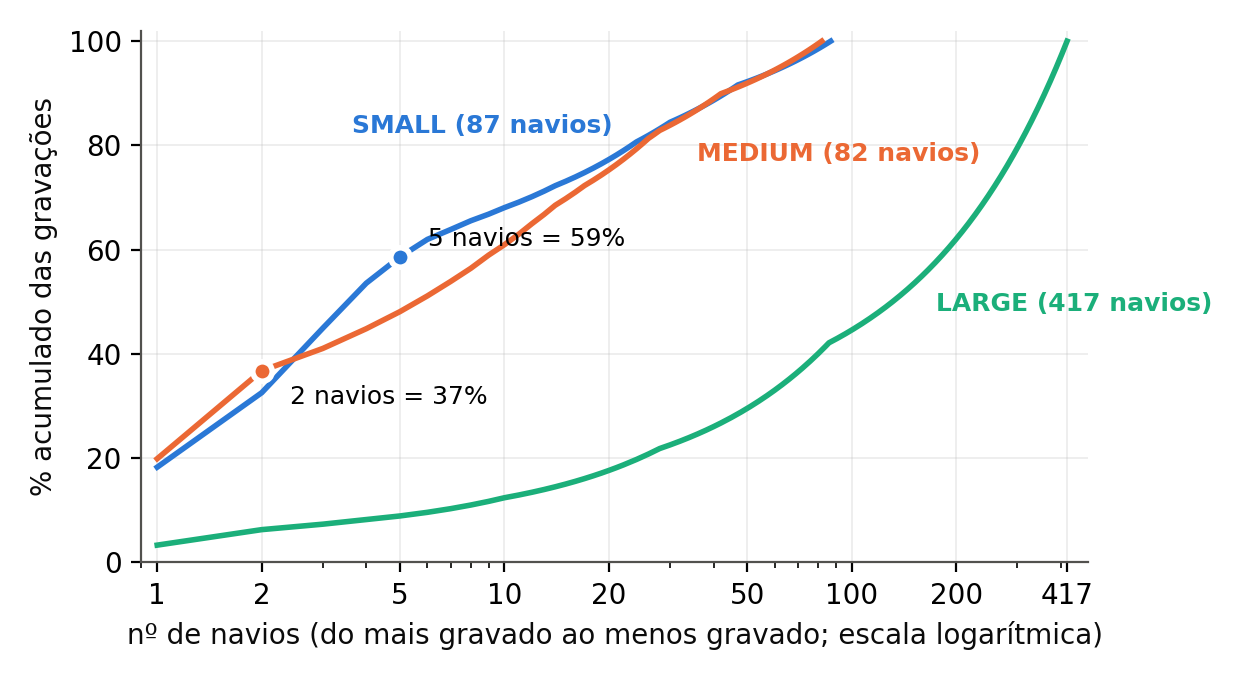
\includegraphics[width=\textwidth]{concentracao_navios.png}
        \column{0.4\textwidth}
        \begin{block}{\small Como ler}
            \scriptsize
            Navios ordenados do mais para o menos gravado (eixo log). Uma curva que sobe rápido = classe dominada por poucos navios.
            \begin{itemize}
                \setlength{\itemsep}{1pt}
                \item SMALL: 5 lanchas de prático (PILOT 08--14) = \textbf{59\%} das gravações.
                \item MEDIUM: 2 dragas irmãs (HANG BO 2002/2003) = \textbf{37\%}.
                \item LARGE: os 5 maiores navios = 8\%.
            \end{itemize}
        \end{block}
    \end{columns}
\end{frame}

\begin{frame}{Composição por Tipo de Navio}
    \centering
    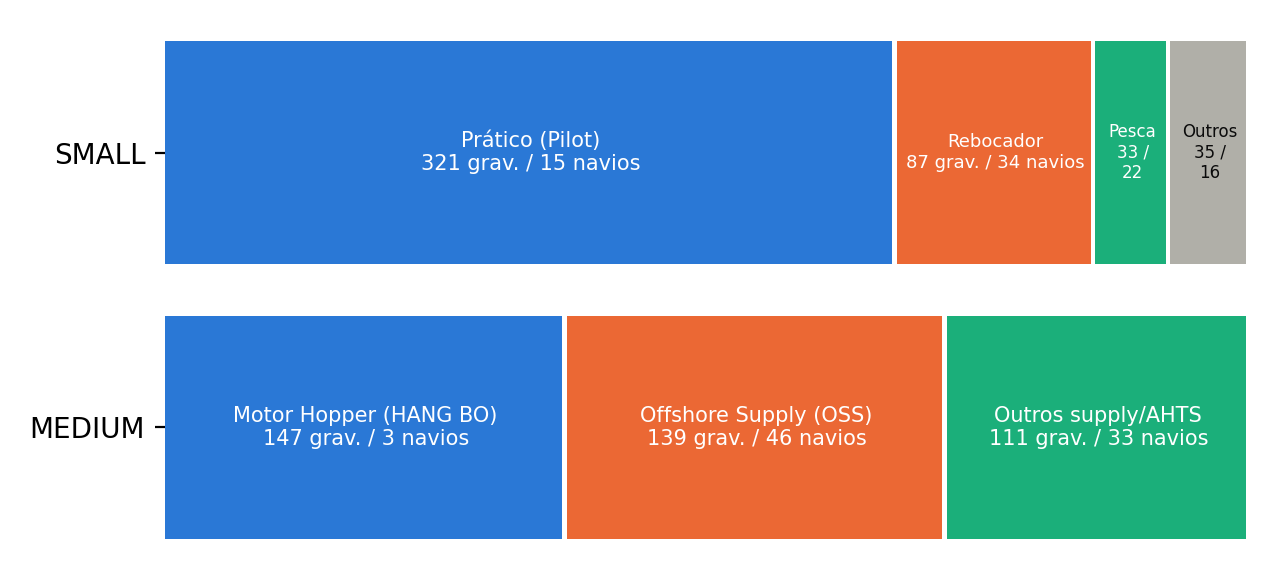
\includegraphics[width=0.74\textwidth]{composicao_tipos.png}

    {\tiny Gravações / navios distintos por tipo (\texttt{DETAILED TYPE} do IARA). ``Outros'' de SMALL: lanchas rápidas, OSS curtos, recreio, amarração; de MEDIUM: Supply, AHTS, Tug/Supply, MPSV, draga.\par}
    \vspace{0.05cm}
    \begin{alertblock}{Leitura}
        \scriptsize
        \textbf{SMALL é, na prática, ``lancha de prático''} (67\% das gravações vêm de 15 lanchas de 11--13 m). \textbf{MEDIUM é ``draga HANG BO + supply''}. Rebocadores (34 navios) e OSS (46 navios) são as subclasses com mais navios distintos, mas têm poucas gravações cada.
    \end{alertblock}
\end{frame}

\begin{frame}{SMALL: 15 Lanchas de Prático = 1 Tipo de Embarcação}
    \footnotesize
    \begin{columns}[t]
        \column{0.44\textwidth}
        \begin{block}{\small As 15 lanchas (todas ``Pilot Vessel'')}
            \tiny
            \centering
            \setlength{\tabcolsep}{3pt}
            \begin{tabular}{lcc}
            \toprule
            Lancha & Compr. & Gravações \\
            \midrule
            PILOT 14 & 12 m & \textbf{87} \\
            PILOT 08 & 12 m & \textbf{68} \\
            PILOT 09 & 12 m & \textbf{59} \\
            PILOT 11 & 13 m & \textbf{41} \\
            PILOT 10 & 11 m & \textbf{24} \\
            RED I & 12 m & 9 \\
            PILOT 20 & 13 m & 8 \\
            PILOT BOAT I & 8 m & 6 \\
            TISSOT RIO, PILOT 02, PILOT 05 & 10--12 m & 4 cada \\
            PILOT 12 / SPARTA MX & 12 m & 3 / 2 \\
            PILOT 01, RED BOAT RJ 07 & 11 m & 1 cada \\
            \bottomrule
            \end{tabular}
        \end{block}
        \column{0.54\textwidth}
        \begin{block}{\small SMALL por tipo (476 gravações, 87 navios)}
            \tiny
            \centering
            \setlength{\tabcolsep}{3pt}
            \begin{tabular}{lcccc}
            \toprule
            Tipo & Navios & Gravações & \% & Grav./navio \\
            \midrule
            Lancha de prático & 15 & 321 & \calo{67} & \calo{21,4} \\
            Rebocador & 34 & 87 & 18 & 2,6 \\
            Pesca & 22 & 33 & 7 & 1,5 \\
            Lancha rápida & 2 & 8 & 2 & 4,0 \\
            OSS curto & 3 & 8 & 2 & 2,7 \\
            Recreio / iate & 5 & 8 & 2 & 1,6 \\
            Amarração / reboque & 4 & 9 & 2 & 2,3 \\
            Passageiros & 2 & 2 & 0,4 & 1,0 \\
            \bottomrule
            \end{tabular}
        \end{block}
    \end{columns}
    \vspace{0.05cm}
    \begin{alertblock}{Leitura}
        \scriptsize
        As 15 lanchas são \textbf{15 embarcações de um único tipo}, quase todas de 11--13 m; a numeração (PILOT 01--20) sugere a mesma operadora. \textbf{5 lanchas (PILOT 08, 09, 10, 11, 14) têm 279 gravações, 59\% de SMALL.} É provável que o modelo aprenda SMALL sobretudo com elas. Rebocadores e pesqueiros trazem 56 navios, mas só 120 gravações.
    \end{alertblock}
\end{frame}

\begin{frame}{Como MEDIUM e LARGE Estão Organizados}
    \footnotesize
    \begin{columns}[t]
        \column{0.49\textwidth}
        \begin{block}{\small MEDIUM por tipo (397 grav., 82 navios)}
            \tiny
            \centering
            \setlength{\tabcolsep}{2.5pt}
            \begin{tabular}{lcccc}
            \toprule
            Tipo & Navios & Grav. & \% & Grav./navio \\
            \midrule
            Draga (Motor Hopper) & 3 & 147 & \calo{37} & \calo{49,0} \\
            Offshore Supply (OSS) & 46 & 139 & 35 & 3,0 \\
            Supply & 7 & 33 & 8 & 4,7 \\
            Anchor Handling (AHTS) & 6 & 32 & 8 & 5,3 \\
            Tug/Supply & 5 & 22 & 6 & 4,4 \\
            Multi Purpose Offshore & 6 & 12 & 3 & 2,0 \\
            Outros (8 tipos) & 9 & 12 & 3 & 1,3 \\
            \bottomrule
            \end{tabular}

            \vspace{0.05cm}
            {\tiny Dragas: HANG BO 2003 (79), HANG BO 2002 (67) e TIGER (1).\par}
        \end{block}
        \column{0.49\textwidth}
        \begin{block}{\small LARGE por tipo (572 grav., 417 navios)}
            \tiny
            \centering
            \setlength{\tabcolsep}{2.5pt}
            \begin{tabular}{lcccc}
            \toprule
            Tipo & Navios & Grav. & \% & Grav./navio \\
            \midrule
            Graneleiro & 161 & 189 & 33 & \cahi{1,2} \\
            Porta-contêiner & 88 & 140 & 24 & \cahi{1,6} \\
            Petroleiro (cru) & 47 & 60 & 10 & \cahi{1,3} \\
            Químico/petroleiro & 37 & 52 & 9 & \cahi{1,4} \\
            Carga geral & 30 & 32 & 6 & \cahi{1,1} \\
            Draga & 4 & 22 & 4 & 5,5 \\
            Outros (10 tipos) & 50 & 77 & 13 & 1,5 \\
            \bottomrule
            \end{tabular}

            \vspace{0.05cm}
            {\tiny Navio mais gravado: PEARL RIVER (draga, 19 gravações, 3\%).\par}
        \end{block}
    \end{columns}
    \vspace{0.1cm}
    \begin{alertblock}{Leitura}
        \scriptsize
        \textbf{MEDIUM = 2 dragas irmãs + navios de apoio offshore.} As HANG BO têm 146 gravações; os 46 OSS, só 3 cada. \textbf{LARGE é o oposto}: 5 tipos com 30 a 161 navios cada e $\sim$1 gravação por navio. LARGE não tem menos tipos; tem \textbf{muitos navios diferentes dentro de cada tipo}, e provavelmente é isso que falta a SMALL e MEDIUM.
    \end{alertblock}
\end{frame}

\begin{frame}{CPA e Distância: Como as Gravações de Navio Foram Selecionadas}
    \footnotesize
    \begin{columns}[T]
        \begin{column}{0.44\textwidth}
            \centering
            \vspace{0.25cm}
            \begin{tikzpicture}[scale=0.52, every node/.style={font=\tiny}]
                % regiões
                \fill[peeblue!8] (0,0) circle (3.0);
                \fill[peeblue!22] (0,0) circle (1.5);
                \draw[peeblue!70, dashed] (0,0) circle (3.0);
                \draw[peeblue!70, dashed] (0,0) circle (1.5);
                \node[peeblue!80!black] at (-0.75,0.75) {250 m};
                \node[peeblue!80!black] at (-1.95,1.6) {500 m};
                % hidrofone
                \fill[black] (0,0) circle (0.11);
                \node[above right] at (0.02,0.02) {hidrofone};
                % rota 1: passa a ~150 m (A ou B)
                \draw[-{Stealth[length=5pt]}, thick, greenwin] (-3.9,-0.9) -- (3.9,-0.9);
                \fill[greenwin] (0,-0.9) circle (0.09);
                \draw[greenwin, densely dotted] (0,0) -- (0,-0.9);
                \node[greenwin, left] at (-0.05,-0.55) {CPA};
                \node[greenwin, anchor=west] at (2.3,-1.25) {A ou B};
                % rota 2: passa a ~350 m (C ou D)
                \draw[-{Stealth[length=5pt]}, thick, orange] (-3.9,2.1) -- (3.9,2.1);
                \fill[orange] (0,2.1) circle (0.09);
                \node[orange, above] at (0.75,2.1) {CPA};
                \node[orange, anchor=west] at (2.3,2.45) {C ou D};
                % rota 3: passa a ~1 km (fora)
                \draw[-{Stealth[length=5pt]}, thick, gray] (-3.9,3.55) -- (3.9,3.55);
                \node[gray, anchor=west] at (1.3,3.85) {a 1 km: fora do IARA (A--E)};
            \end{tikzpicture}\\[2pt]
            \scriptsize
            \setlength{\tabcolsep}{4pt}
            \begin{tabular}{@{}lcc@{}}
                \toprule
                & Tem o CPA & Não tem o CPA \\
                \midrule
                até 250 m & \textbf{A} & \textbf{B} \\
                250--500 m & \textbf{C} & \textbf{D} \\
                \bottomrule
            \end{tabular}
        \end{column}
        \begin{column}{0.54\textwidth}
            \begin{block}{\small O que é o CPA}
                \scriptsize
                \textit{Closest Point of Approach}: o \textbf{ponto da rota do navio mais perto do hidrofone} e o instante em que ele passa por ali. O hidrofone fica parado no fundo; o navio se aproxima, passa pelo CPA e se afasta, então a distância muda ao longo da gravação e o som costuma ser mais forte no CPA.
            \end{block}
            \begin{block}{\small Como a distância define o subconjunto}
                \scriptsize
                \begin{itemize}
                    \setlength{\itemsep}{1pt}
                    \item Raio medido \textbf{até o hidrofone}, pelo AIS: \textbf{A e B} = navio a até 250 m; \textbf{C e D} = entre 250 e 500 m.
                    \item \textbf{A e C:} a gravação inclui o CPA. \textbf{B e D:} foi cortada antes ou depois dele (outro navio entraria a menos de 2 km).
                \end{itemize}
            \end{block}
        \end{column}
    \end{columns}
\end{frame}

\begin{frame}{Distância e CPA: Iguais nas Duas Classes}
    \footnotesize
    \begin{columns}[t]
        \column{0.44\textwidth}
        \begin{block}{\small Gravações por subconjunto}
            \scriptsize
            \centering
            \begin{tabular}{lcccc}
            \toprule
             & A & B & C & D \\
            \midrule
            SMALL & 113 & 90 & 104 & 169 \\
            MEDIUM & 120 & 73 & 75 & 129 \\
            LARGE & 223 & 36 & 162 & 151 \\
            \bottomrule
            \end{tabular}

            \vspace{0.05cm}
            {\tiny A/B até 250 m, C/D 250--500 m; A/C contêm o CPA, B/D não. Com CPA: SMALL 46\%, MEDIUM 49\%, LARGE 67\%.\par}
        \end{block}
        \column{0.54\textwidth}
        \begin{block}{\small Recall (\%) por subconjunto}
            \scriptsize
            \centering
            \setlength{\tabcolsep}{4pt}
            \begin{tabular}{llcccc}
            \toprule
            Modelo & Classe & A & B & C & D \\
            \midrule
            \multirow{2}{*}{CNN LOFAR (gravação)} & SMALL & 48 & 49 & 46 & 48 \\
             & MEDIUM & 76 & 61 & 56 & 60 \\
            \midrule
            \multirow{2}{*}{MLP LOFAR (navio)} & SMALL & 55 & 41 & 52 & 47 \\
             & MEDIUM & 36 & 30 & 31 & 31 \\
            \bottomrule
            \end{tabular}
        \end{block}
    \end{columns}
    \vspace{0.1cm}
    \begin{alertblock}{Leitura}
        \scriptsize
        SMALL e MEDIUM têm a mesma distribuição de distância e de CPA, e o acerto quase não muda entre subconjuntos (B, sem CPA e perto, é o pior). \textbf{Distância e geometria da passagem não parecem explicar} a confusão SMALL/MEDIUM. Em LARGE, ao contrário, o CPA pesava muito (82\% das acertadas $\times$ 33\% das erradas).
    \end{alertblock}
\end{frame}

%===========================================
% SEÇÃO 3
%===========================================
\section{As Extrações}

\begin{frame}
    \centering
    \huge As Extrações
\end{frame}

\begin{frame}{LOFAR: Como É Calculado}
    \footnotesize
    \begin{columns}[T]
        \begin{column}{0.55\textwidth}
            \begin{block}{\small Passos (pipeline do projeto)}
                \scriptsize
                \begin{enumerate}
                    \setlength{\itemsep}{1pt}
                    \item \textbf{Decimação por 3:} 48 kHz $\to$ 16 kHz (filtro anti-aliasing; o sinal fica atenuado acima de $\sim$6,4 kHz).
                    \item \textbf{Espectrograma:} FFT de 2.048 pontos com janela de Hann, sem sobreposição $\to$ quadros de 0,128 s e \textbf{1.024 faixas de 7,8 Hz} (0--8 kHz).
                    \item \textbf{Integração:} média de 4 quadros $\to$ um espectro a cada \textbf{0,512 s}.
                    \item \textbf{Log:} 20$\cdot$log$_{10}$ da magnitude.
                    \item \textbf{TPSW:} subtrai o fundo local estimado em cada faixa (média de $\pm$4 a $\pm$21 faixas, ou seja, $\pm$31 a $\pm$164 Hz, ignorando o centro; 2 passadas com corte em 2$\times$). Valores abaixo de $-$0,2 dB viram 0.
                    \item \textbf{Para os modelos:} normalização L2 por espectro; a MLP usa a média de 10 quadros (\textbf{janelas de 5,12 s}) e a gravação recebe o voto da maioria das janelas.
                \end{enumerate}
            \end{block}
        \end{column}
        \begin{column}{0.43\textwidth}
            \begin{block}{\small O que o TPSW faz, em palavras}
                \scriptsize
                Compara cada faixa com a vizinhança de $\pm$160 Hz. Uma linha estreita ou uma banda de até $\sim$60 Hz de largura se destaca; um ruído que sobe devagar por centenas de Hz vira ``fundo'' e some.
            \end{block}
            \begin{block}{\small Consequências}
                \scriptsize
                \begin{itemize}
                    \setlength{\itemsep}{1pt}
                    \item A ``energia'' do LOFAR é \textbf{contraste local}, não relação sinal-ruído.
                    \item O nível absoluto e a inclinação do espectro \textbf{se perdem}.
                    \item Abaixo de $\sim$150 Hz o TPSW tem pouca vizinhança à esquerda: ler com cautela.
                \end{itemize}
            \end{block}
        \end{column}
    \end{columns}
\end{frame}

\begin{frame}{DEMON: Como É Calculado}
    \footnotesize
    \begin{columns}[T]
        \begin{column}{0.55\textwidth}
            \begin{block}{\small Passos (pipeline do projeto)}
                \scriptsize
                \begin{enumerate}
                    \setlength{\itemsep}{1pt}
                    \item Passa-faixa de \textbf{1--2 kHz} (Chebyshev II): isola o ruído de cavitação.
                    \item \textbf{Envelope} pelo valor absoluto (retificação).
                    \item Decimação até \textbf{50 Hz} (enxerga modulações até 25 Hz); o envelope é dividido pelo seu pico (sem nível absoluto).
                    \item STFT de 512 pontos com 50\% de sobreposição $\to$ janelas de \textbf{10,24 s} a cada 5,12 s; 4 faixas de DC descartadas $\to$ \textbf{253 faixas de 0,098 Hz}, de 0,4 a 25 Hz.
                    \item Nas análises: dB acima do fundo TPSW ($\pm$1,56 Hz, sem as $\pm$0,29 Hz centrais); pico procurado só a partir de 1 Hz.
                \end{enumerate}
            \end{block}
        \end{column}
        \begin{column}{0.43\textwidth}
            \begin{block}{\small O que o DEMON faz, em palavras}
                \scriptsize
                A hélice ``liga e desliga'' o ruído de cavitação a cada volta e a cada pá. O DEMON mede o ritmo dessa modulação.\\[3pt]
                Uma hélice de 4 pás a 150 rpm dá linhas em \textbf{2,5 Hz} (eixo) e \textbf{10 Hz} (pás).
            \end{block}
        \end{column}
    \end{columns}
\end{frame}

\begin{frame}{MEL e HHT: Como São Calculados}
    \footnotesize
    \vspace{-4pt}
    \begin{columns}[T]
        \begin{column}{0.49\textwidth}
            \begin{block}{\small MEL (entrada da CNN MEL)}
                \scriptsize
                \begin{enumerate}
                    \setlength{\itemsep}{1pt}
                    \item \textbf{Decimação por 3:} 48 kHz $\to$ 16 kHz (mesmo filtro do LOFAR; atenuado acima de $\sim$6,4 kHz).
                    \item \textbf{Espectrograma de potência:} FFT de 2.048 pontos, janela de Hann, sem sobreposição $\to$ quadros de 0,128 s.
                    \item \textbf{Banco mel:} \textbf{256 bandas de 0 a 8 kHz} (Slaney): espaçadas de 11,7 Hz até 1 kHz (85 bandas), depois cada vez mais largas, até $\sim$96 Hz em 8 kHz.
                    \item \textbf{dB relativo ao máximo da gravação} (piso em $-$80 dB): não é nível absoluto.
                    \item \textbf{Integração:} média de 4 quadros $\to$ um espectro a cada \textbf{0,512 s}.
                    \item \textbf{Sem TPSW}; para os modelos, \textbf{L2 por espectro}, como no LOFAR.
                \end{enumerate}
            \end{block}
        \end{column}
        \begin{column}{0.49\textwidth}
            \begin{block}{\small HHT (Hilbert--Huang; extração do projeto)}
                \scriptsize
                \begin{enumerate}
                    \setlength{\itemsep}{1pt}
                    \item \textbf{Decimação por 24:} 48 kHz $\to$ \textbf{2 kHz} (FIR, fase zero) $\to$ só \textbf{1--1.000 Hz}. Sinal com média 0 e desvio 1.
                    \item \textbf{Janelas de 2,56 s a cada 5,12 s}: metade do áudio fica de fora.
                    \item \textbf{EMD:} cada janela vira até \textbf{8 modos} (IMFs), 30 iterações de peneiramento.
                    \item \textbf{Hilbert:} a energia instantânea (amplitude$^2$) de cada modo é somada na faixa da sua frequência instantânea.
                    \item \textbf{HHT 1D:} \textbf{256 faixas de 3,9 Hz}, dividido pelo pico da janela.
                    \item \textbf{HHT 2D:} \textbf{32 passos de 80 ms $\times$ 128 faixas de 7,9 Hz}, log(1+x), dividido pelo pico da janela.                \end{enumerate}
            \end{block}
        \end{column}
    \end{columns}
\end{frame}

%===========================================
% SEÇÃO 4
%===========================================
\section{Os Modelos Generalizam?}

\begin{frame}
    \centering
    \huge Os Modelos Generalizam?
\end{frame}

\begin{frame}{Split por Navio: MEDIUM Desaba, SMALL Quase Não Muda}
    \footnotesize
    \begin{table}
    \centering
    \scriptsize
    \setlength{\tabcolsep}{4pt}
    \begin{tabular}{lcccccc}
    \toprule
     & \multicolumn{3}{c}{Split por gravação (artigo)} & \multicolumn{3}{c}{Split por navio} \\
    \cmidrule(lr){2-4}\cmidrule(lr){5-7}
    Modelo & SP & SMALL & MEDIUM & SP & SMALL & MEDIUM \\
    \midrule
    MLP LOFAR & 67,4 & 54,1 & 65,9 & 56,1 & 49,8 & \calo{34,5} \\
    SVM MEL & 61,3 & 53,6 & 52,5 & 50,5 & 47,0 & \calo{31,4} \\
    BiGRU LOFAR & 62,5 & 57,5 & 50,5 & 50,8 & 47,0 & \calo{27,6} \\
    \bottomrule
    \end{tabular}
    \end{table}
    {\tiny Mesmo código, sementes e tamanho de treino; só muda a regra de divisão (NB29, \texttt{reports/split\_navio/folds.csv}). Acaso com 4 classes = 25\%.\par}
    \vspace{0.1cm}
    \begin{alertblock}{Leitura}
        \scriptsize
        \textbf{Não, para MEDIUM}: em navios nunca vistos o recall fica entre 28\% e 35\%, perto do acaso. O SP cai 11 pontos. \textbf{SMALL generaliza pouco, mas generaliza}: perde só 4--10 pontos e fica em $\sim$47--50\%. O SP do artigo provavelmente mede, em boa parte, reconhecimento de navios repetidos.
    \end{alertblock}
\end{frame}

\begin{frame}{MEDIUM Acertadas: Padrão ou Navios Conhecidos?}
    \footnotesize
    \begin{columns}[t]
        \column{0.55\textwidth}
        \begin{block}{\small Acerto da CNN LOFAR pelo nº de gravações do navio}
            \scriptsize
            \centering
            \begin{tabular}{lccc}
            \toprule
            Gravações do navio & MEDIUM & SMALL & LARGE \\
            \midrule
            1 & \calo{25\%} & 20\% & 63\% \\
            2--3 & 32\% & 29\% & 56\% \\
            4--10 & 31\% & 26\% & 46\% \\
            mais de 10 & \cahi{64\%} & 26\% & 69\% \\
            \bottomrule
            \end{tabular}

            \vspace{0.05cm}
            {\tiny \% de gravações acertadas em todos os folds.\par}
        \end{block}
        \column{0.43\textwidth}
        \begin{block}{\small Concentração}
            \scriptsize
            \begin{itemize}
                \setlength{\itemsep}{1pt}
                \item 138 das 193 MEDIUM acertadas (\textbf{72\%}) vêm de 7 navios gravados mais de 10 vezes.
                \item 2 Motor Hoppers irmãos (HANG BO 2002/2003) somam \textbf{37\%} das gravações MEDIUM.
                \item O split do artigo é \textbf{por gravação}: em todo fold, $\sim$25--35 gravações do HANG BO 2003 estão no teste e o resto no treino.
            \end{itemize}
        \end{block}
    \end{columns}
    \vspace{0.1cm}
    \begin{alertblock}{Leitura}
        \scriptsize
        O acerto em MEDIUM parece vir mais de \textbf{reconhecer navios já vistos} do que de um padrão de frequência. Em LARGE, a curva é plana: lá o acerto se mantém em navios novos. Em SMALL, o acerto é baixo mesmo para navios conhecidos.
    \end{alertblock}
\end{frame}

\begin{frame}{Com Split por Navio, MEDIUM Desaba em Todos os Modelos}
    \footnotesize
    \begin{columns}[t]
        \column{0.55\textwidth}
        \begin{block}{\small Recall de MEDIUM: split por gravação $\to$ por navio (NB29)}
            \scriptsize
            \centering
            \begin{tabular}{lcc}
            \toprule
            Modelo & Recall MEDIUM (\%) & Acc. bal. \\
            \midrule
            SVM MEL & 52,5 $\to$ \calo{31,4} & $-8{,}6$ \\
            SVM LOFAR & 55,0 $\to$ \calo{32,9} & $-5{,}4$ \\
            MLP MEL & 68,5 $\to$ \calo{41,0} & $-8{,}5$ \\
            MLP LOFAR & 65,9 $\to$ \calo{34,5} & $-9{,}6$ \\
            RF MEL & 51,9 $\to$ \calo{29,2} & $-9{,}5$ \\
            RF LOFAR & 40,0 $\to$ \calo{23,1} & $-8{,}4$ \\
            BiGRU LOFAR & 50,5 $\to$ \calo{27,6} & $-9{,}2$ \\
            \bottomrule
            \end{tabular}

            \vspace{0.05cm}
            {\tiny Mesmo código e sementes; só muda a regra de divisão. Queda média: MEDIUM $-23$ p.p., SMALL $-5{,}5$, LARGE $-3{,}4$, BACKGROUND $-0{,}2$.\par}
        \end{block}
        \column{0.43\textwidth}
        \begin{block}{\small Motor Hoppers irmãos (split por navio)}
            \scriptsize
            \centering
            Reconhecidos como MEDIUM:

            \vspace{0.05cm}
            \begin{tabular}{lcc}
            \toprule
            Modelo & Irmão no treino & Nenhum \\
            \midrule
            MLP LOFAR & 77\% & 8\% \\
            MLP MEL & 71\% & 13\% \\
            SVM MEL & 64\% & 2\% \\
            BiGRU LOFAR & 57\% & 7\% \\
            RF LOFAR & 54\% & 0\% \\
            \bottomrule
            \end{tabular}
        \end{block}
    \end{columns}
    \vspace{0.1cm}
    \begin{alertblock}{Leitura}
        \scriptsize
        Em navios novos, MEDIUM fica entre 23\% e 41\% (acaso com 4 classes: 25\%). Tudo indica que os modelos aprendem a \textbf{identidade do navio ou da série} (``este é um HANG BO''), e não a \textbf{classe de tamanho}. Como acontece nos 7 modelos, o problema parece estar mais no dado do que na capacidade do modelo.
    \end{alertblock}
\end{frame}

\begin{frame}{LARGE e BACKGROUND: Generalizam}
    \footnotesize
    \begin{columns}[T]
        \begin{column}{0.50\textwidth}
            \begin{block}{\small Recall (\%) gravação $\to$ navio}
                \scriptsize
                \centering
                \setlength{\tabcolsep}{4pt}
                \begin{tabular}{lcc}
                \toprule
                Modelo & LARGE & BACKGROUND \\
                \midrule
                MLP LOFAR & 71,2 $\to$ \cahi{67,7} & 80,0 $\to$ \cahi{81,1} \\
                SVM MEL & 71,5 $\to$ \cahi{67,0} & 72,5 $\to$ \cahi{70,3} \\
                BiGRU LOFAR & 68,1 $\to$ \cahi{66,2} & 75,8 $\to$ \cahi{74,3} \\
                \bottomrule
                \end{tabular}\\[3pt]
                {\tiny Mesmos modelos e folds do slide anterior. Acaso = 25\%.\par}
            \end{block}
        \end{column}
        \begin{column}{0.48\textwidth}
            \begin{block}{\small Por que quase não muda}
                \scriptsize
                \begin{itemize}
                    \setlength{\itemsep}{2pt}
                    \item \textbf{LARGE:} 417 navios, a maioria com uma só gravação. No split do artigo, só 29\% dos LARGE de teste já tinham o navio no treino: para LARGE, o split do artigo já era quase ``por navio''.
                    \item \textbf{BACKGROUND:} não tem navio; cada gravação é o seu próprio grupo nos dois splits. A diferença ($\pm$2 pontos) deve vir de treinos diferentes.
                \end{itemize}
            \end{block}
        \end{column}
    \end{columns}
    \vspace{0.1cm}
    \begin{alertblock}{Leitura}
        \scriptsize
        \textbf{Sim, LARGE e BACKGROUND generalizam}: em navios nunca vistos, o LARGE perde só 2--5 pontos e fica em 66--68\%; o BACKGROUND acerta 70--81\% de gravações nunca vistas. O que mais acompanha o acerto do LARGE é \textbf{mais energia em $\sim$50 Hz que as outras classes} (próximos slides). Mas não é exclusivo: SMALL e MEDIUM também têm energia ali, em geral menos, e as gravações deles que chegam ao nível do LARGE tendem a ser confundidas com LARGE.
    \end{alertblock}
\end{frame}

\begin{frame}{LARGE Acertadas: Corcova Grave (Média de 346 Gravações)}
    \begin{columns}[c]
        \begin{column}{0.56\textwidth}
            \centering
            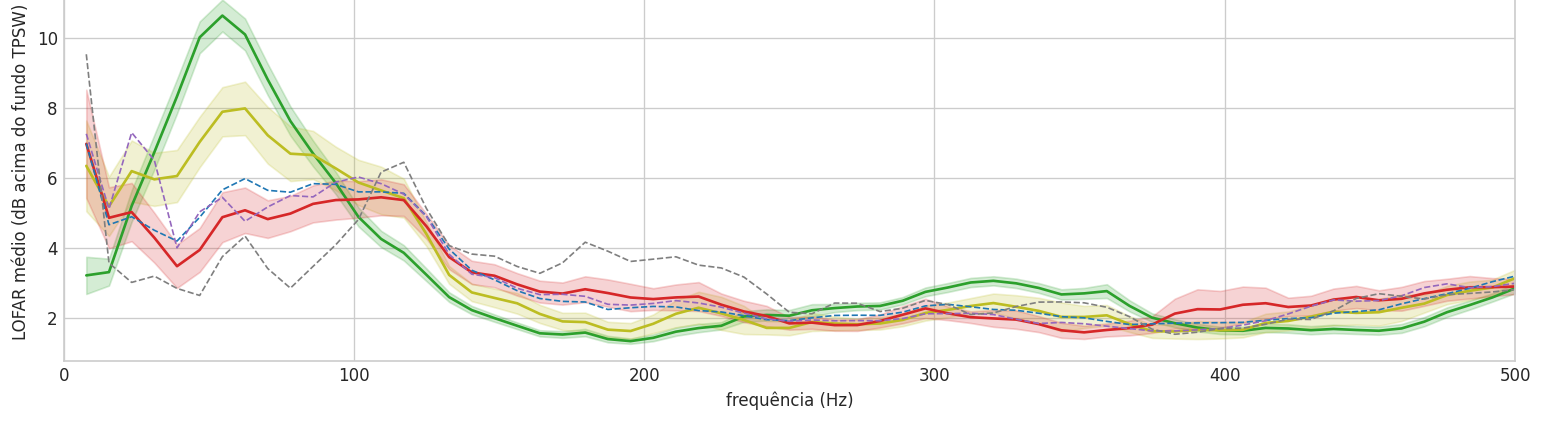
\includegraphics[width=\textwidth]{lofar_large_espectro_zoom.png}\\
            {\tiny Espectro LOFAR médio, 0--500 Hz. Tracejadas: SMALL (azul), MEDIUM (roxo), BACKGROUND (cinza).\\
            \textbf{Faixa colorida = intervalo de confiança de 95\% da média}, em cada frequência: média $\pm$ 1,96 $\times$ desvio padrão $\div \sqrt{n}$. Mostra a incerteza da \textbf{média}, não a variação entre gravações (próximo slide); é estreita porque $n$ é grande.\par}
        \end{column}
        \begin{column}{0.42\textwidth}
            \begin{block}{\small Os grupos (CNN LOFAR)}
                \tiny
                Cada gravação foi testada $\sim$5 vezes (folds diferentes).\\[2pt]
                \setlength{\tabcolsep}{2pt}
                \begin{tabular}{@{}l>{\raggedright\arraybackslash}p{2.6cm}r@{}}
                \toprule
                Grupo & O que aconteceu nos $\sim$5 testes & Grav. \\
                \midrule
                \textcolor{greenwin}{\textbf{Verde:}} acertadas & disse LARGE em todos & 346 \\
                \textcolor{goldencolor}{\textbf{Amarelo:}} oscilam & às vezes disse LARGE, às vezes não (ex.: 3 de 5) & 109 \\
                \textcolor{red}{\textbf{Vermelho:}} erradas & nunca disse LARGE & 117 \\
                \bottomrule
                \end{tabular}
            \end{block}
        \end{column}
    \end{columns}
    \vspace{0.05cm}
    \begin{alertblock}{Leitura}
        \scriptsize
        \begin{itemize}
            \setlength{\itemsep}{1pt}
            \item \textbf{Acertadas:} um pico alto em $\sim$55 Hz, 10,7 dB acima do fundo. \textbf{Erradas:} quase sem pico (4,9 dB). \textbf{Oscilam:} no meio, e o modelo fica em dúvida.
            \item Em 47 Hz, comparando uma acertada com uma errada, a acertada tem mais energia em \textbf{89\% dos pares}.
            \item \textbf{As LARGE erradas parecem SMALL}: a curva vermelha fica quase em cima da azul tracejada.
            \item Vale \textbf{dentro de cada subconjunto} A--D: não é só efeito de distância ou de CPA.
        \end{itemize}
    \end{alertblock}
\end{frame}

\begin{frame}{LARGE: Uma Linha por Gravação}
    \centering
    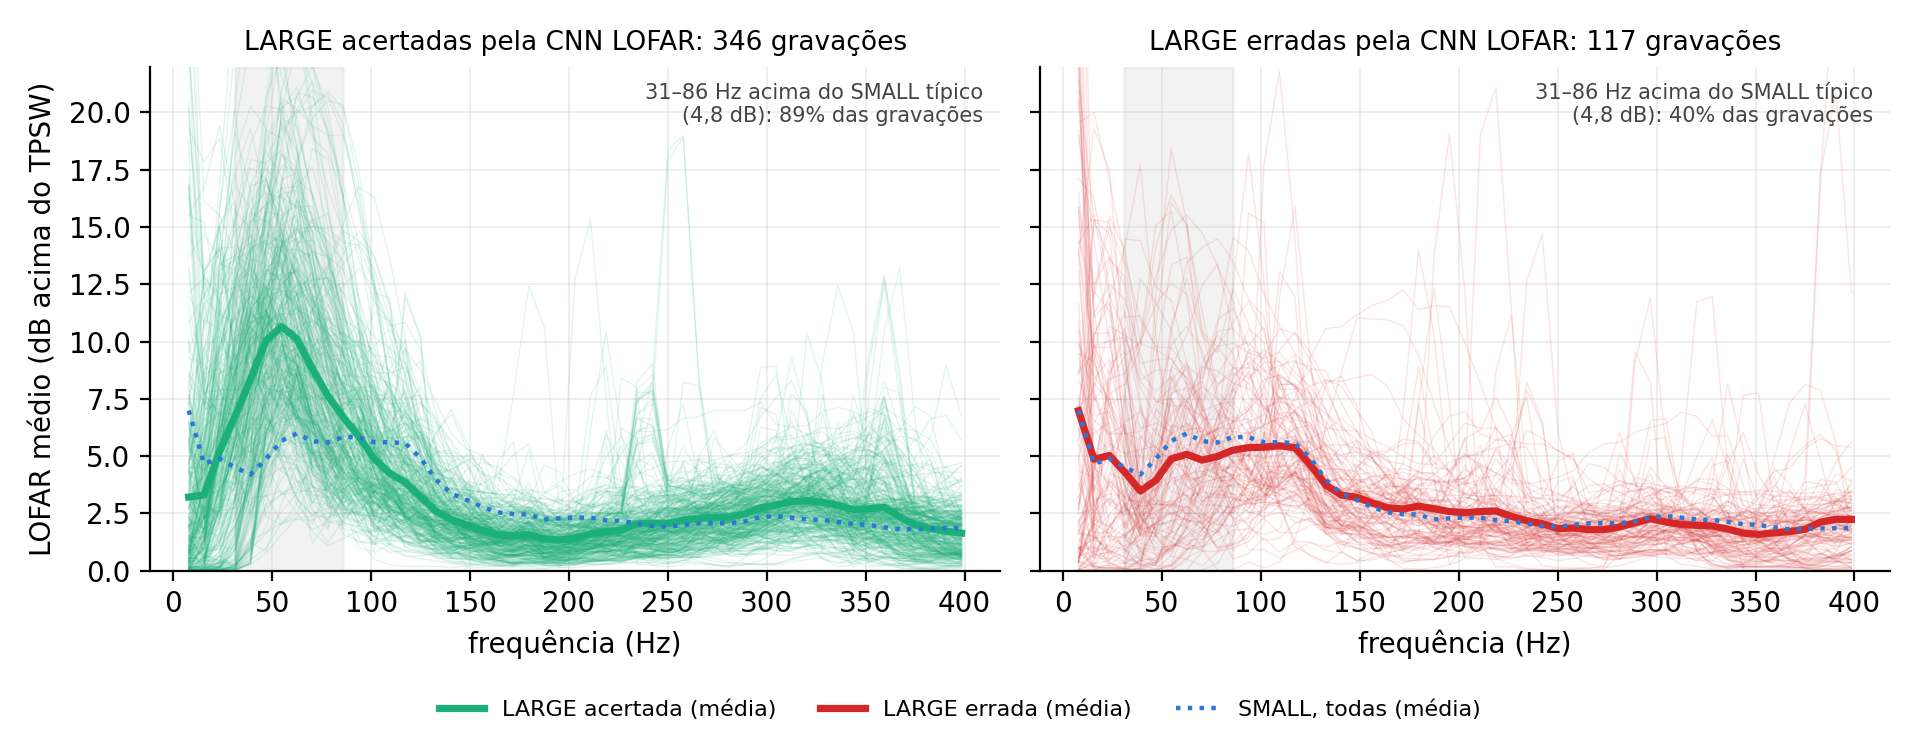
\includegraphics[width=0.80\textwidth]{large_uma_linha.png}

    {\tiny Mesmos grupos do slide anterior (CNN LOFAR do artigo; acertada = acerta em todos os testes, errada = erra em todos; as 109 que oscilam ficam de fora). Cada linha fina é uma gravação; a grossa é a média. Faixa cinza = 31--86 Hz.\par}
    \vspace{0.05cm}
    \begin{alertblock}{Leitura}
        \scriptsize
        \textbf{Acertadas:} \textbf{89\%} têm o grave de 31--86 Hz acima do SMALL típico (mediana 8,4 dB), mas variam muito, de $\sim$2 a 20 dB. \textbf{Erradas:} a média fica quase em cima da do SMALL (mediana 4,2 dB); ainda assim, 40\% têm grave acima do SMALL típico. A média do slide anterior resume bem a tendência, mas \textbf{não é uma regra}: há LARGE acertadas sem corcova e erradas com ela.
    \end{alertblock}
\end{frame}

\begin{frame}{LARGE no MEL: Uma Linha por Gravação}
    \centering
    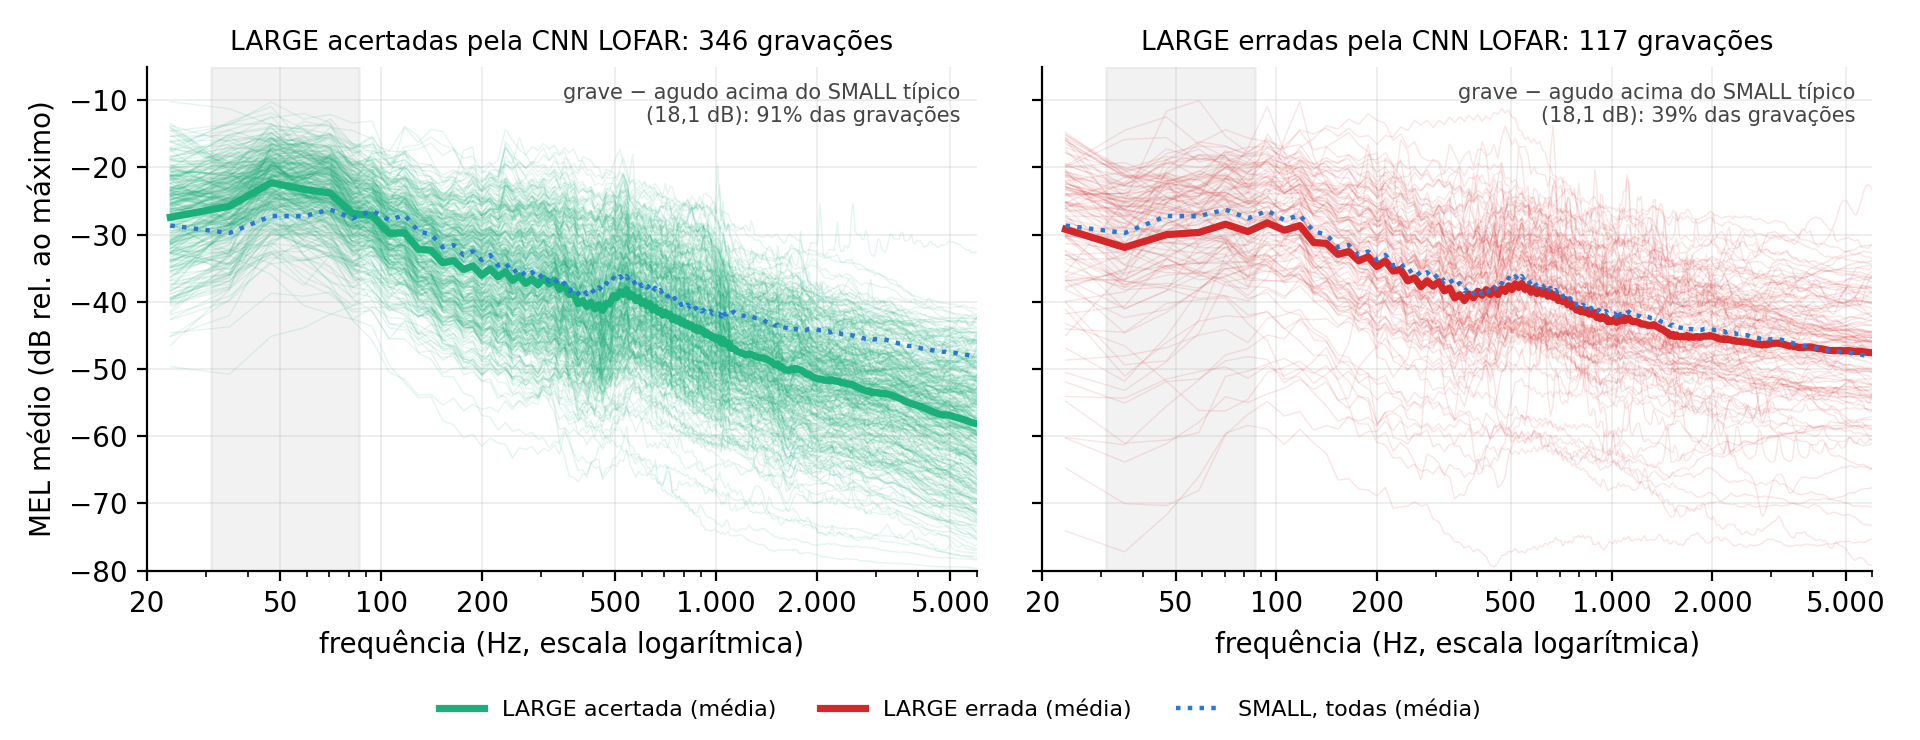
\includegraphics[width=0.66\textwidth]{large_uma_linha_mel.png}

    {\tiny Mesmos grupos do slide anterior (CNN LOFAR). MEL sem normalização (dB relativo ao ponto mais forte da gravação; sem TPSW). \textbf{Grave $-$ agudo} = média de 31--86 Hz menos média de 1--6 kHz: quanto o grave domina o agudo. SMALL típico = mediana das gravações SMALL (18,1 dB).\par}
    \vspace{0.02cm}
    \begin{alertblock}{Leitura}
        \scriptsize
        \begin{itemize}
            \setlength{\itemsep}{1pt}
            \item \textbf{Acertadas:} um pouco mais de grave e \textbf{bem menos agudo} que as erradas. Em \textbf{87\% dos pares}, a acertada tem o grave mais dominante; 91\% ficam acima do SMALL típico.
            \item \textbf{Erradas:} a média fica quase em cima da do SMALL, como no LOFAR. Só 39\% ficam acima do SMALL típico.
            \item O MEL é uma medida que a CNN LOFAR nunca viu e \textbf{reforça o LOFAR}: a LARGE errada tende a soar como SMALL.
        \end{itemize}
    \end{alertblock}
\end{frame}

\begin{frame}{LARGE no DEMON: Uma Linha por Gravação}
    \centering
    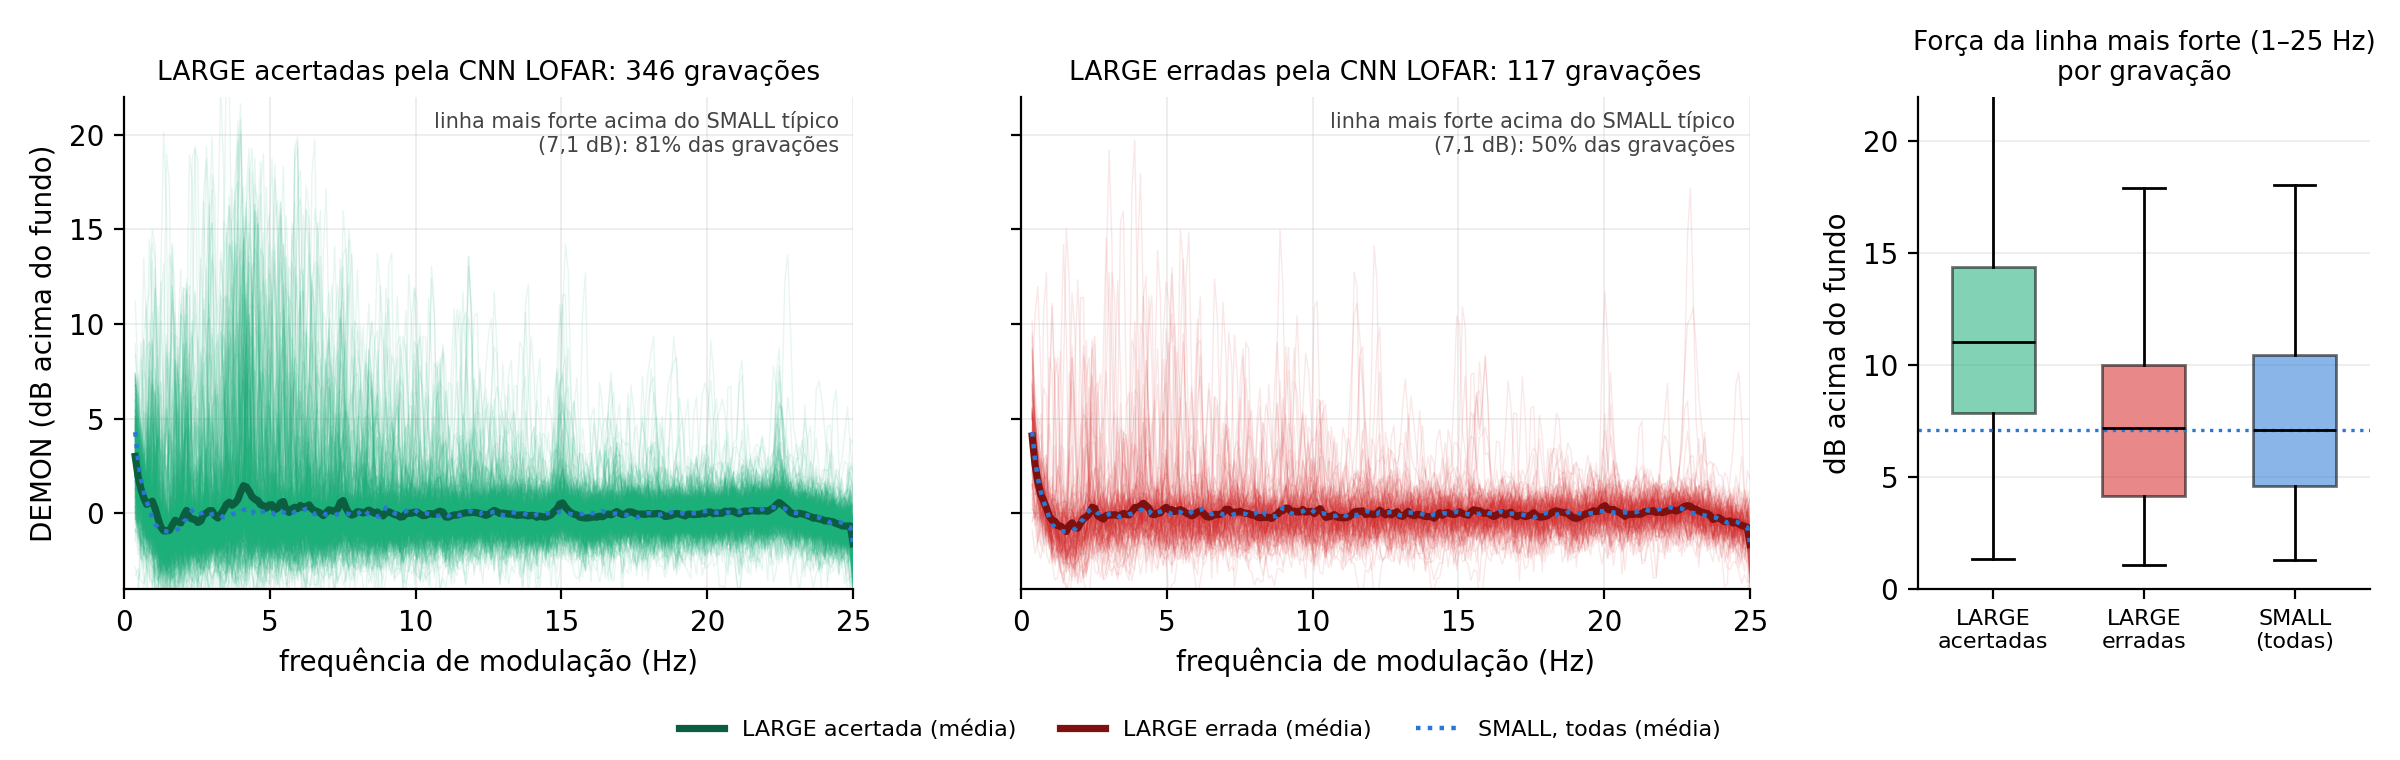
\includegraphics[width=0.70\textwidth]{large_uma_linha_demon.png}

    {\tiny Mesmos grupos dos slides anteriores (CNN LOFAR). DEMON da banda de 1--2 kHz, em dB acima do fundo: a hélice gera \textbf{picos (``linhas'')} no ritmo do eixo e das pás.\\
    \textbf{Força da linha mais forte} = altura do \textbf{pico mais alto} de cada linha fina, entre 1 e 25 Hz. Pico alto = ritmo da hélice bem marcado. Boxplot: linha preta = mediana; caixa = metade central das gravações; pontilhado azul = SMALL típico (7,1 dB).\par}
    \vspace{0.02cm}
    \begin{alertblock}{Leitura}
        \scriptsize
        \begin{itemize}
            \setlength{\itemsep}{1pt}
            \item \textbf{Nas linhas, os dois grupos parecem iguais}: cada navio tem o ritmo numa frequência diferente, e as médias ficam planas.
            \item \textbf{No boxplot aparece a diferença}: as acertadas têm a linha mais forte (11,1 dB típico, contra 7,2 dB); as erradas ficam iguais ao SMALL.
            \item \textbf{É uma diferença moderada}: a acertada tem a linha mais forte em 73\% dos pares (no LOFAR e no MEL, 87--89\%), e as caixas se sobrepõem.
        \end{itemize}
    \end{alertblock}
\end{frame}

\begin{frame}{Exemplos de Espectrogramas LOFAR (LARGE)}
    \centering
    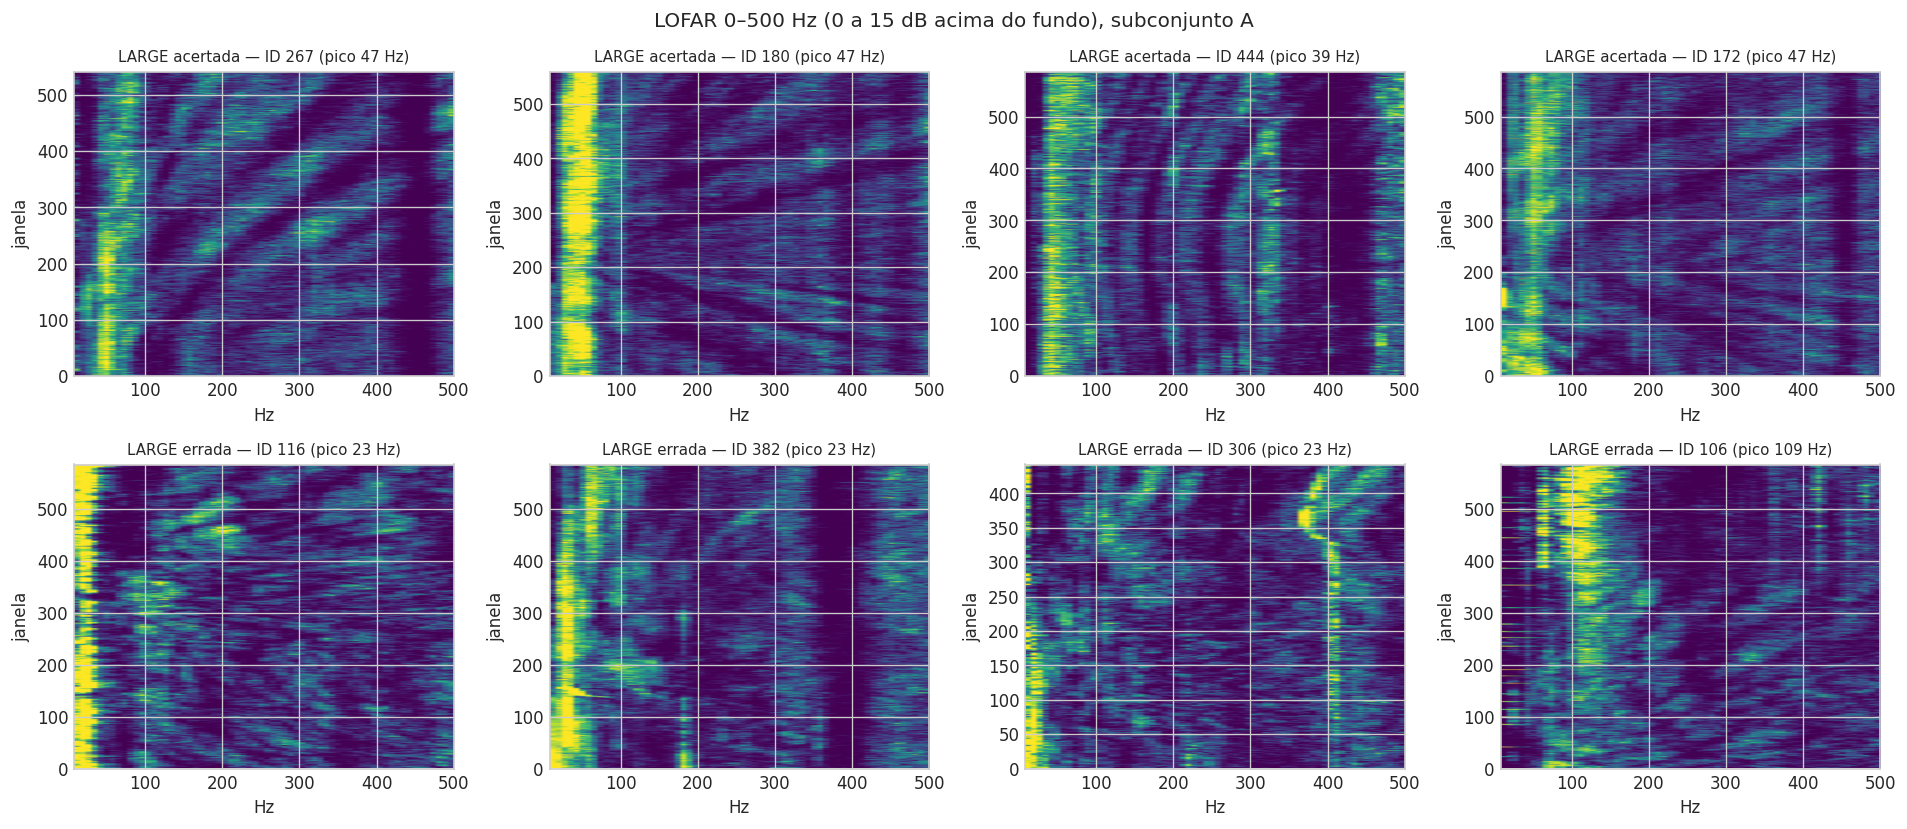
\includegraphics[width=0.95\textwidth]{lofar_large_exemplos.png}

    {\tiny Subconjunto A, 0--500 Hz, 0 a 15 dB acima do fundo. Linha de cima: acertadas (banda clara e estável em $\sim$30--80 Hz). Linha de baixo: erradas (energia abaixo de $\sim$30 Hz ou acima de $\sim$90 Hz).\par}
\end{frame}

\begin{frame}{Por Tipo de Navio: Quem Sustenta o Acerto}
    \footnotesize
    \begin{columns}[t]
        \column{0.49\textwidth}
        \begin{block}{\small SMALL: recall (\%) gravação $\to$ navio}
            \scriptsize
            \centering
            \setlength{\tabcolsep}{3pt}
            \begin{tabular}{lccc}
            \toprule
            Tipo (navios) & MLP LOFAR & SVM MEL & BiGRU \\
            \midrule
            Prático (15) & 55 $\to$ 49 & 56 $\to$ 43 & 58 $\to$ 43 \\
            Rebocador (34) & 49 $\to$ 45 & 49 $\to$ 44 & 54 $\to$ 45 \\
            Pesca (22) & 51 $\to$ 50 & 44 $\to$ 47 & 47 $\to$ 43 \\
            \bottomrule
            \end{tabular}
        \end{block}
        \column{0.49\textwidth}
        \begin{block}{\small MEDIUM: recall (\%) gravação $\to$ navio}
            \scriptsize
            \centering
            \setlength{\tabcolsep}{3pt}
            \begin{tabular}{lccc}
            \toprule
            Tipo (navios) & MLP LOFAR & SVM MEL & BiGRU \\
            \midrule
            Motor Hopper (3) & \cahi{89} $\to$ \calo{36} & 78 $\to$ \calo{27} & 81 $\to$ \calo{27} \\
            OSS (46) & 51 $\to$ 32 & 37 $\to$ 29 & 32 $\to$ 25 \\
            Outros supply (33) & 54 $\to$ 29 & 38 $\to$ 31 & 33 $\to$ 20 \\
            \bottomrule
            \end{tabular}
        \end{block}
    \end{columns}
    \vspace{0.1cm}
    \begin{block}{\small Para onde vão os erros (split por navio)}
        \scriptsize
        SMALL errada $\to$ LARGE 45--56\%, MEDIUM 38--45\%, BG 5--10\%. \quad MEDIUM errada $\to$ \textbf{SMALL 65--75\%}, LARGE 23--33\%.
    \end{block}
    \vspace{0.05cm}
    \begin{alertblock}{Leitura}
        \scriptsize
        O MEDIUM ``bom'' do artigo era o Motor Hopper (89\%), que é reconhecido quase só quando o irmão está no treino. Para navios novos, \textbf{MEDIUM vira SMALL}: o modelo não parece ter aprendido algo que separe um supply de 80 m de um rebocador de 30 m. Em SMALL, o acerto é parecido nos três tipos: pode haver algum padrão comum, fraco.
    \end{alertblock}
\end{frame}

%===========================================
% SEÇÃO 5
%===========================================
\section{Condições de Gravação}

\begin{frame}
    \centering
    \huge Condições de Gravação
\end{frame}

\begin{frame}{Os LARGE Foram Gravados com o Mar Mais Calmo}
    \begin{columns}[c]
        \column{0.58\textwidth}
        \centering
        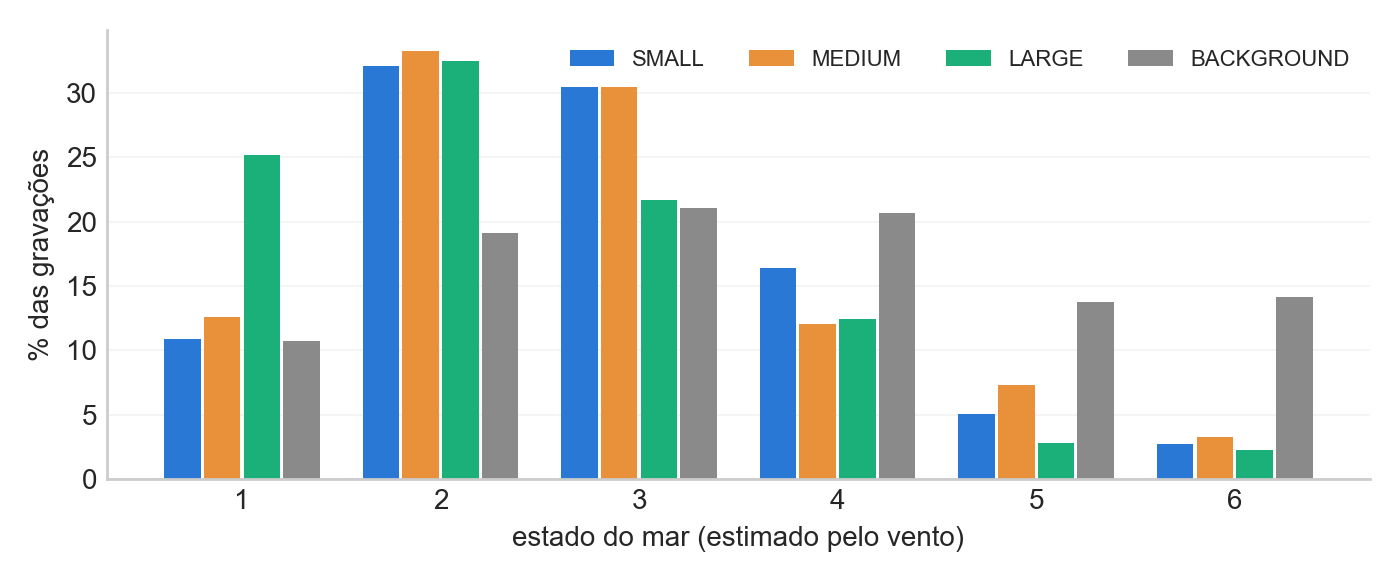
\includegraphics[width=\textwidth]{mar_por_classe.png}
        \column{0.4\textwidth}
        \begin{block}{\small Por gravação}
            \tiny
            \centering
            \setlength{\tabcolsep}{3pt}
            \begin{tabular}{lccc}
            \toprule
             & Vento & Mar calmo & Chuva \\
             & (m/s) & (estado $\leq$ 2) & \\
            \midrule
            SMALL & 4,8 & 43\% & 8\% \\
            MEDIUM & 4,7 & 46\% & 5\% \\
            LARGE & \cahi{3,8} & \cahi{58\%} & 7\% \\
            BACKGROUND & 6,8 & 30\% & \calo{42\%} \\
            \bottomrule
            \end{tabular}
        \end{block}
    \end{columns}
    \vspace{0.05cm}
    \begin{alertblock}{Leitura}
        \scriptsize
        Por navio, a diferença é significativa entre LARGE e os navios $<$ 100 m (p $<$ 0,001), mas não entre SMALL e MEDIUM (p = 0,71). \textbf{É um viés da base}: com condições iguais, a separação entre as classes provavelmente seria um pouco menor. Chuva quase só aparece no BACKGROUND, que foi escolhido em condições variadas.
    \end{alertblock}
\end{frame}

\begin{frame}{O BACKGROUND Cobre Mar Agitado}
    \footnotesize
    \begin{columns}[t]
        \column{0.55\textwidth}
        \begin{block}{\small BACKGROUND (subconjunto E): estado do mar $\times$ chuva}
            \tiny
            \centering
            \setlength{\tabcolsep}{4pt}
            \begin{tabular}{lcccc}
            \toprule
            Estado do mar & Sem chuva & Com chuva & Total \\
            \midrule
            1 & 25 & 3 & 28 \\
            2 & 25 & 25 & 50 \\
            3 & 25 & 30 & 55 \\
            4 & \cahi{25} & 29 & 54 \\
            5 & \cahi{25} & 11 & 36 \\
            6 & \cahi{25} & 12 & 37 \\
            7 & \cahi{1} & 0 & 1 \\
            \bottomrule
            \end{tabular}
        \end{block}
        \column{0.43\textwidth}
        \begin{block}{\small Desenho proposital}
            \scriptsize
            \begin{itemize}
                \setlength{\itemsep}{1pt}
                \item 25 gravações sem chuva \textbf{em cada estado do mar} de 1 a 6.
                \item Vento de 1,3 a 20 m/s.
                \item Nenhum navio num raio de 10 km.
                \item 76 fundos sem chuva com mar $\geq$ 4; 50 com mar $\leq$ 2.
            \end{itemize}
        \end{block}
    \end{columns}
    \begin{alertblock}{Leitura}
        \scriptsize
        Há material para ``sujar'' gravações LARGE de mar calmo com ruído real de mar agitado. Os LARGE, ao contrário, têm só 29 gravações com mar 5 ou 6.
    \end{alertblock}
\end{frame}

\begin{frame}{A MLP Erra Mais LARGE com o Mar Agitado}
    \begin{columns}[c]
        \column{0.58\textwidth}
        \centering
        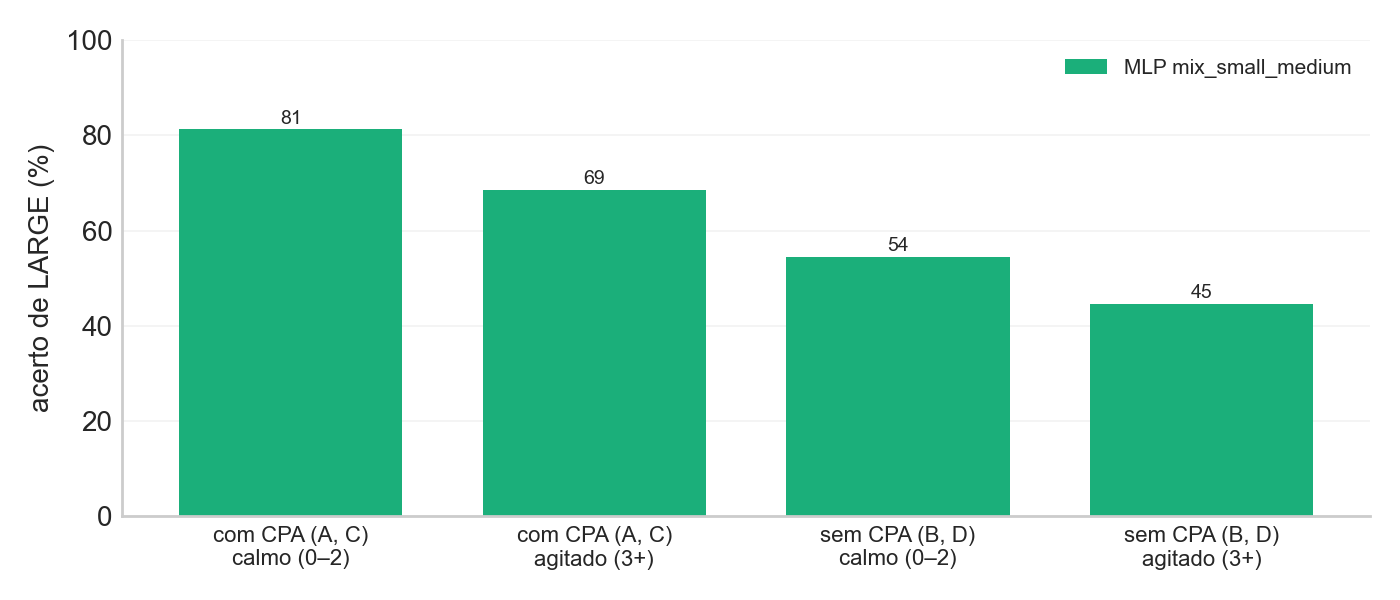
\includegraphics[width=\textwidth]{large_cpa_mar.png}

        {\tiny MLP mix\_small\_medium (NB40), split por navio.\par}
        \column{0.4\textwidth}
        \begin{block}{\small Faixa 31--86 Hz (dB acima do fundo)}
            \tiny
            \centering
            \begin{tabular}{lcc}
            \toprule
             & Calmo & Agitado \\
            \midrule
            Com CPA & 8,0 & 7,1 \\
            Sem CPA & 7,0 & 5,8 \\
            \bottomrule
            \end{tabular}
        \end{block}
        \begin{block}{\small \texttt{MIX\_SMALL\_MEDIUM} com CPA}
            \tiny
            Calmo 77\% $\rightarrow$ agitado 75\%: quase não sofre.
        \end{block}
    \end{columns}
    \vspace{0.05cm}
    \begin{alertblock}{Leitura}
        \scriptsize
        \textbf{O mar agitado tira $\sim$10 pontos do acerto de LARGE, com ou sem CPA}; o pior caso (sem CPA e agitado) acerta só 45\%. Provavelmente o ruído do mar sobe e o grave do navio se destaca menos do fundo. Vento e estado do mar vêm de estação próxima, não do local.
    \end{alertblock}
\end{frame}

%===========================================
% SEÇÃO 6
%===========================================
\section{O Que Falta: Navios ou Gravações?}

\begin{frame}
    \centering
    \huge O Que Falta: Navios ou Gravações?
\end{frame}

\begin{frame}{Curva de Aprendizado pelo Número de Navios}
    \begin{columns}[c]
        \column{0.6\textwidth}
        \centering
        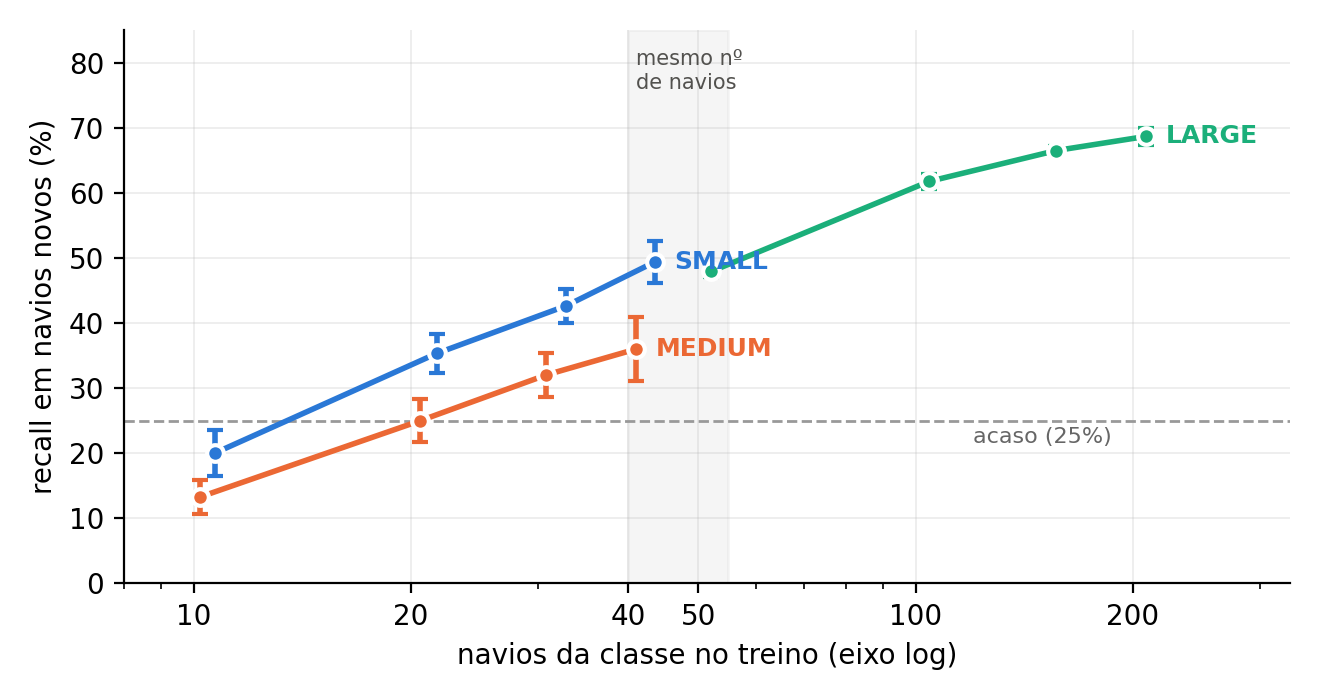
\includegraphics[width=\textwidth]{curva_navios.png}
        \column{0.38\textwidth}
        \begin{block}{\small Como foi feito}
            \tiny
            Em cada fold do split por navio, mantive no treino 25, 50, 75 ou 100\% dos navios de SMALL e MEDIUM (controle: só de LARGE) e medi o recall em navios nunca vistos. MLP LOFAR, 10 folds $\times$ 2 sorteios.
        \end{block}
        \begin{block}{\small Recall em navios novos}
            \tiny
            \centering
            \setlength{\tabcolsep}{3pt}
            \begin{tabular}{lcccc}
            \toprule
            SMALL (navios) & 11 & 22 & 33 & 44 \\
            recall (\%) & 20 & 35 & 43 & 49 \\
            \midrule
            MEDIUM (navios) & 11 & 22 & 33 & 44 \\
            recall (\%) & 13 & 25 & 32 & 36 \\
            \midrule
            LARGE (navios) & 52 & 104 & 156 & 208 \\
            recall (\%) & 48 & 62 & 67 & 69 \\
            \bottomrule
            \end{tabular}
        \end{block}
    \end{columns}
    \vspace{0.05cm}
    \begin{alertblock}{Leitura}
        \scriptsize
        Nenhuma curva estabilizou: cada vez que o nº de navios dobra, o recall sobe $\sim$14 pontos (SMALL) e $\sim$11 (MEDIUM). \textbf{Com o mesmo nº de navios, SMALL acerta como LARGE} (49\% com 44 navios $\times$ 48\% com 52). LARGE não parece ser ``mais fácil''; o que provavelmente ajuda é ter mais navios.
    \end{alertblock}
\end{frame}

\begin{frame}{Muitas Gravações do Mesmo Navio Ajudam?}
    \footnotesize
    \begin{columns}[t]
        \column{0.5\textwidth}
        \begin{block}{\small Recall (\%) pelo nº de gravações do navio (MLP LOFAR)}
            \scriptsize
            \centering
            \setlength{\tabcolsep}{3pt}
            \begin{tabular}{lcccc}
            \toprule
             & \multicolumn{2}{c}{SMALL} & \multicolumn{2}{c}{MEDIUM} \\
            \cmidrule(lr){2-3}\cmidrule(lr){4-5}
            Gravações & gravação & navio & gravação & navio \\
            \midrule
            1 (40 navios) & 46 & 45 & 35 & 30 \\
            2--3 & 61 & 53 & 53 & 37 \\
            4--9 & 59 & 55 & 54 & 34 \\
            10+ & 52 & 47 & \cahi{77} & \calo{32} \\
            \bottomrule
            \end{tabular}

            \vspace{0.05cm}
            {\tiny ``gravação'' = split do artigo (o navio pode estar no treino); ``navio'' = split por navio (nunca visto).\par}
        \end{block}
        \column{0.48\textwidth}
        \begin{block}{\small Navios mais gravados: gravação $\to$ navio}
            \scriptsize
            \centering
            \setlength{\tabcolsep}{3pt}
            \begin{tabular}{lcc}
            \toprule
            Navio (gravações) & recall (\%) \\
            \midrule
            HANG BO 2002 (67) & \cahi{89} $\to$ \calo{36} \\
            HANG BO 2003 (79) & \cahi{89} $\to$ \calo{36} \\
            NORMAND PIONEER (10) & 76 $\to$ 32 \\
            PILOT 08 (68) & 60 $\to$ 52 \\
            PILOT 14 (87) & 56 $\to$ 47 \\
            PILOT 10 (24) & 33 $\to$ 37 \\
            \bottomrule
            \end{tabular}
        \end{block}
    \end{columns}
    \vspace{0.1cm}
    \begin{alertblock}{Leitura}
        \scriptsize
        \textbf{MEDIUM: o modelo parece decorar o navio.} Com o navio no treino, 77--89\%; nunca visto, $\sim$32\%, com 1 ou com 80 gravações. \textbf{SMALL: nem conhecendo a lancha o acerto sobe} (lanchas de prático com 24--87 gravações ficam em 33--60\%). Tudo indica que falta diversidade de navios, mais do que de gravações.
    \end{alertblock}
\end{frame}

%===========================================
% SEÇÃO 7
%===========================================
\section{Lanchas de Prático e Fronteira de 50 m}

\begin{frame}
    \centering
    \huge Lanchas de Prático e Fronteira de 50 m
\end{frame}

\begin{frame}{Lanchas de Prático: Erradas Mesmo Conhecidas}
    \begin{columns}[c]
        \column{0.6\textwidth}
        \centering
        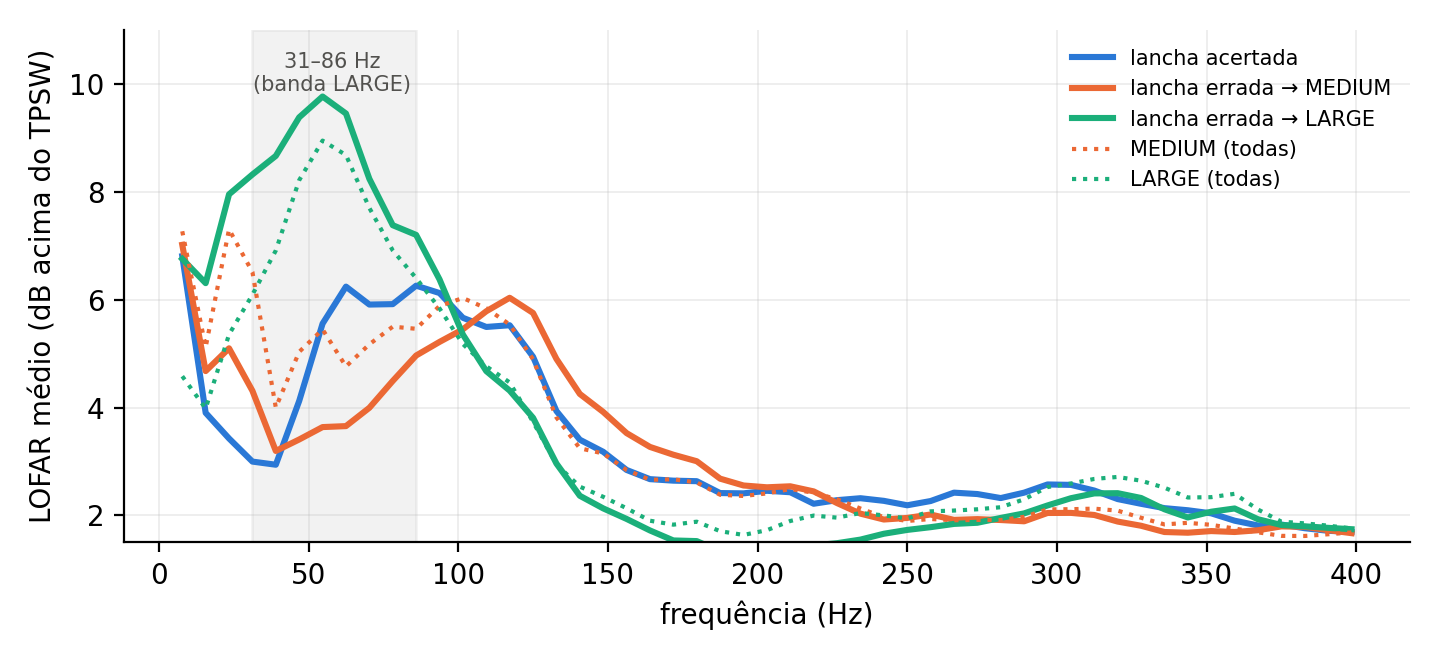
\includegraphics[width=\textwidth]{lancha_espectro.png}
        \column{0.38\textwidth}
        \begin{block}{\small 321 gravações, 15 lanchas}
            \tiny
            Split do artigo (a lancha está no treino). Errada = acertada em menos da metade das 5 vezes em que foi testada.
            \begin{itemize}
                \setlength{\itemsep}{0pt}
                \item acertadas: 175
                \item erradas $\to$ MEDIUM: 77
                \item erradas $\to$ LARGE: 69
            \end{itemize}
            Pior subconjunto: B (59\% erradas; A, C, D: 39--44\%).
        \end{block}
    \end{columns}
    \vspace{0.05cm}
    \begin{alertblock}{Leitura}
        \scriptsize
        As lanchas erradas como LARGE têm \textbf{graves fortes em 31--86 Hz}, mais até que a média das LARGE: a mesma banda que caracteriza LARGE (NB35). Como cada gravação tem uma só embarcação, a origem desses graves não é outro navio, e não dá para identificá-la com os dados do IARA.
    \end{alertblock}
\end{frame}

\begin{frame}{Lanchas Erradas: Uma Linha por Gravação}
    \centering
    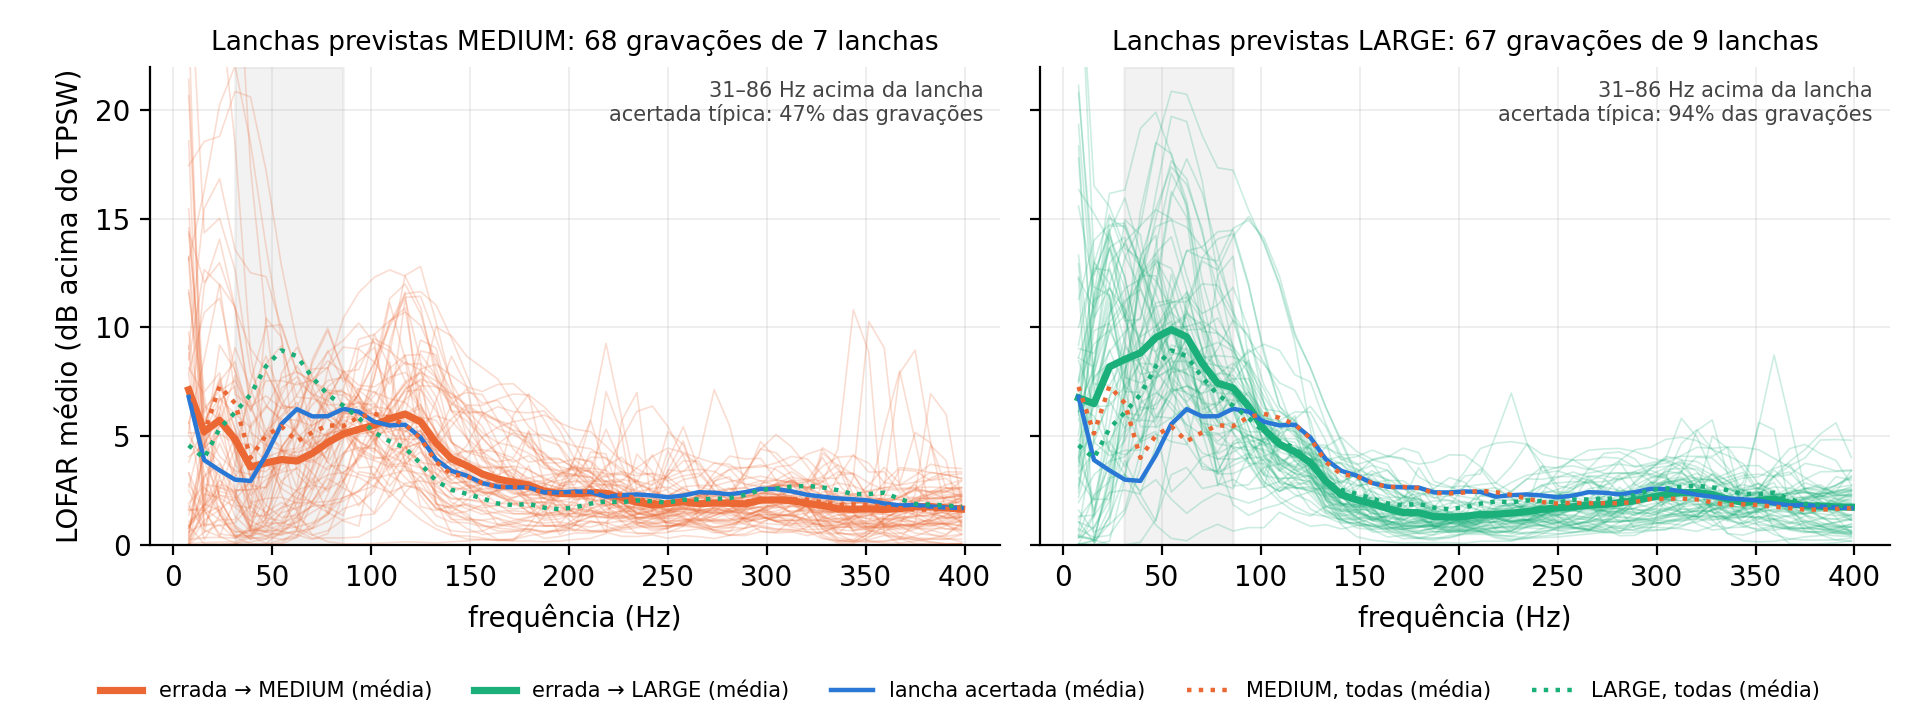
\includegraphics[width=0.86\textwidth]{lanchas_erradas.png}

    {\tiny Classe prevista = a mais votada entre MEDIUM, LARGE e BACKGROUND (11 erradas foram para BACKGROUND e não aparecem). Por isso os totais diferem um pouco do slide anterior, que dividia só entre MEDIUM e LARGE.\par}
    \vspace{0.05cm}
    \begin{alertblock}{Leitura}
        \scriptsize
        \textbf{Erradas $\to$ LARGE:} quase todas (94\%) têm o grave de 31--86 Hz acima da lancha acertada típica, com a corcova no mesmo lugar da média LARGE. \textbf{Erradas $\to$ MEDIUM:} bem mais variadas; na média, o grave em 40--90 Hz \emph{cai} e o pico se desloca para $\sim$100--130 Hz, a faixa de pico mais comum dos MEDIUM. O erro acompanha \textbf{onde fica o pico}.
    \end{alertblock}
\end{frame}

\begin{frame}{Lanchas Acertadas: Uma Linha por Gravação}
    \centering
    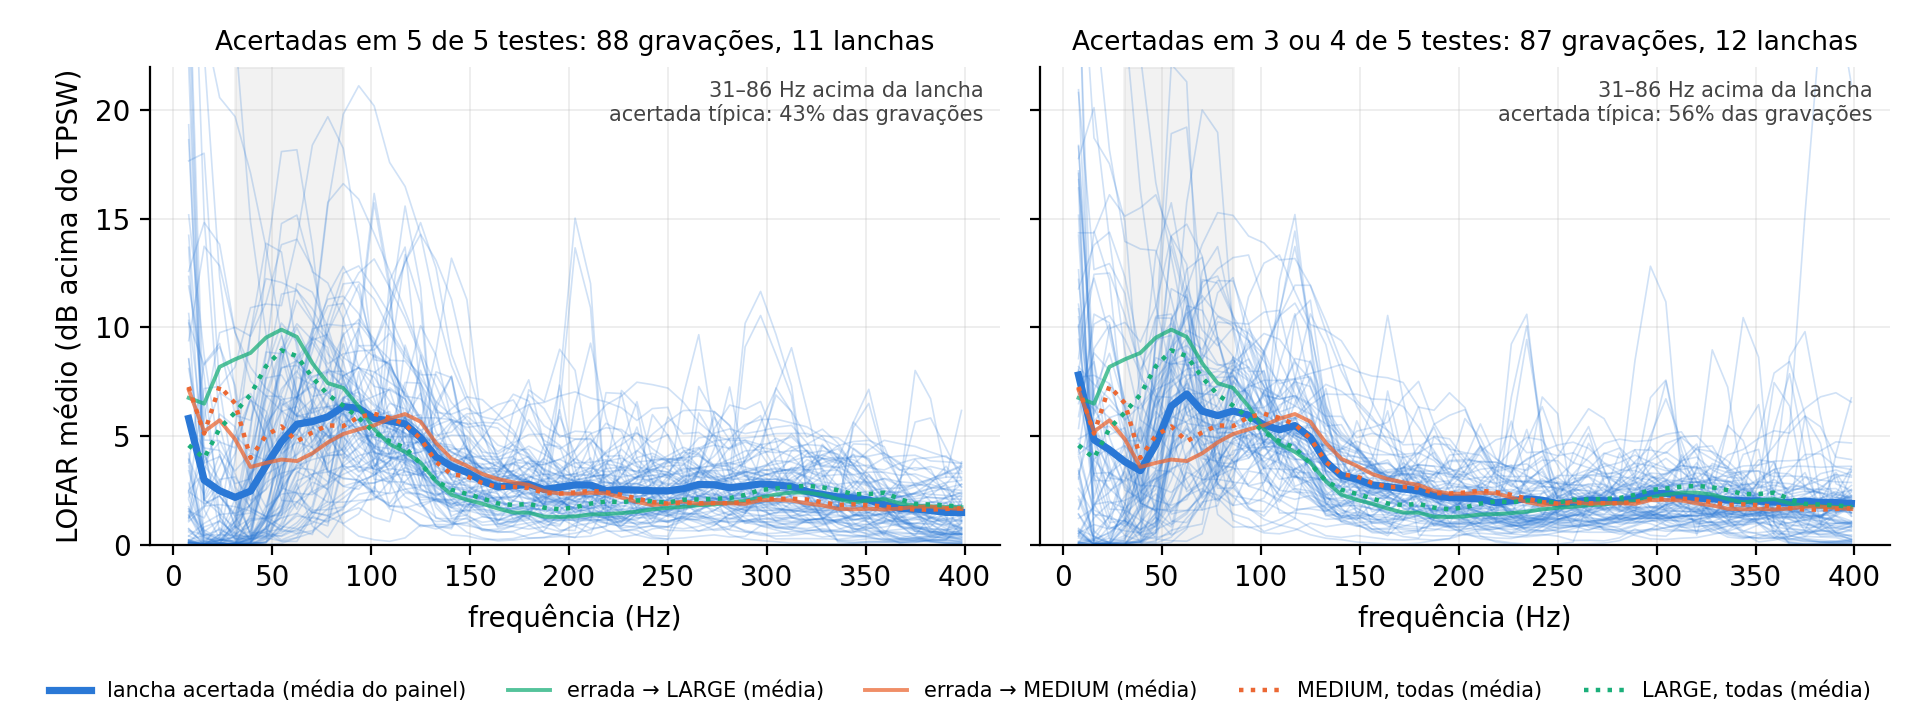
\includegraphics[width=0.86\textwidth]{lanchas_acertadas.png}

    {\tiny MLP LOFAR de 4 classes, split por gravação, \textbf{todos os 10 folds} (5 repetições $\times$ 2): cada gravação é testada 5 vezes. Acertada = classificada SMALL em pelo menos 3 dos 5 testes (175 de 321 gravações de lancha).\par}
    \vspace{0.05cm}
    \begin{alertblock}{Leitura}
        \scriptsize
        \textbf{Acertadas em 5 de 5:} grave fraco em 30--45 Hz e uma subida \emph{larga} até um platô em $\sim$60--120 Hz, sem a corcova estreita dos LARGE em 50--60 Hz. \textbf{Acertadas em 3--4 de 5:} já aparece um pico em $\sim$60 Hz (31--86 Hz: 5,4 contra 4,6 dB), a meio caminho do LARGE --- são as gravações em que o modelo oscila. Mais grave concentrado = menos certeza de SMALL.
    \end{alertblock}
\end{frame}

\begin{frame}{As Mesmas Lanchas no DEMON: Médias por Grupo}
    \centering
    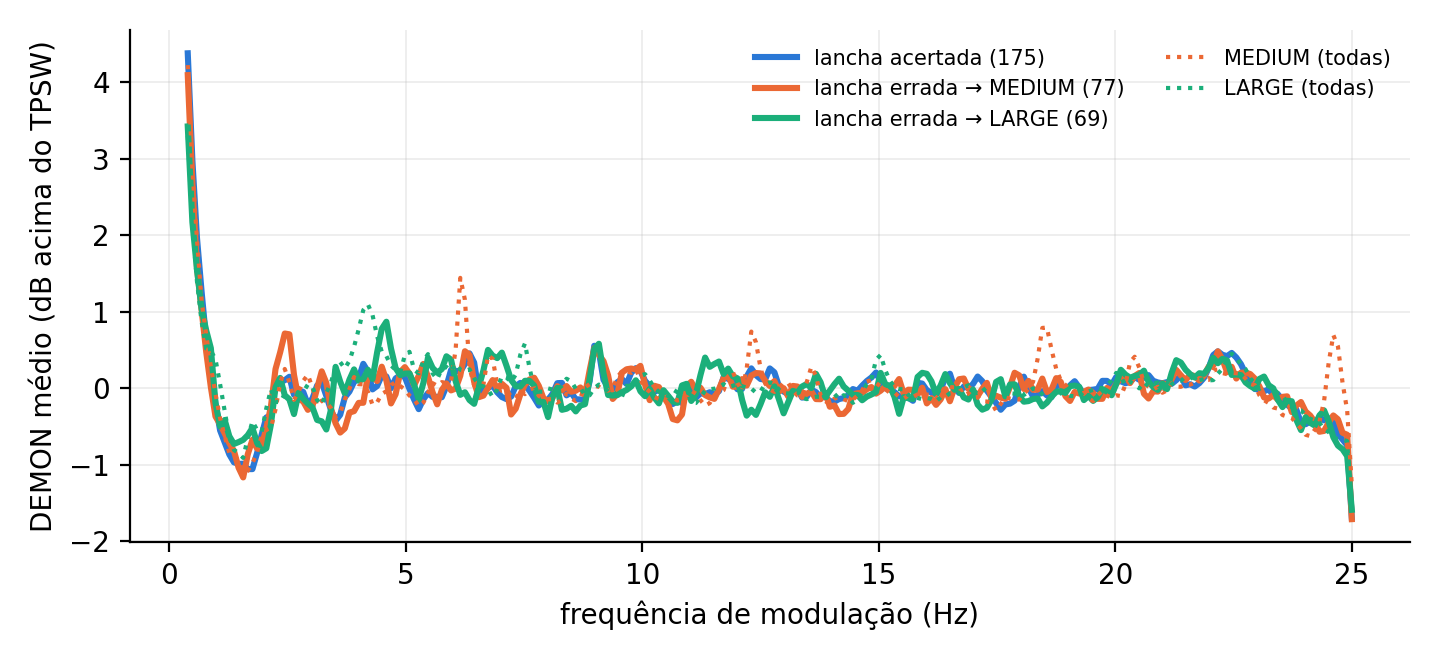
\includegraphics[width=0.66\textwidth]{demon_lancha_espectro.png}

    {\tiny Grupos dos slides anteriores (acertos/erros da MLP \textbf{LOFAR}, split por gravação, todos os folds). DEMON = espectro do envelope da banda 1--2 kHz (ritmos de eixo e pás), em \textbf{dB acima do fundo TPSW} ao longo das frequências de modulação, como no LOFAR. Sem o TPSW, o DEMON do pipeline tem escala arbitrária (envelope dividido pelo próprio pico da gravação).\par}
    \vspace{0.05cm}
    \begin{alertblock}{Leitura}
        \scriptsize
        Na média, os três grupos de lanchas são praticamente iguais: cada lancha tem as suas linhas em frequências diferentes, e a média as apaga. O DEMON não mostra um ``ritmo de LARGE'' nas lanchas erradas como o LOFAR mostrava o grave de 31--86 Hz.
    \end{alertblock}
\end{frame}

\begin{frame}{As Mesmas Lanchas no DEMON: Força da Linha Mais Forte}
    \centering
    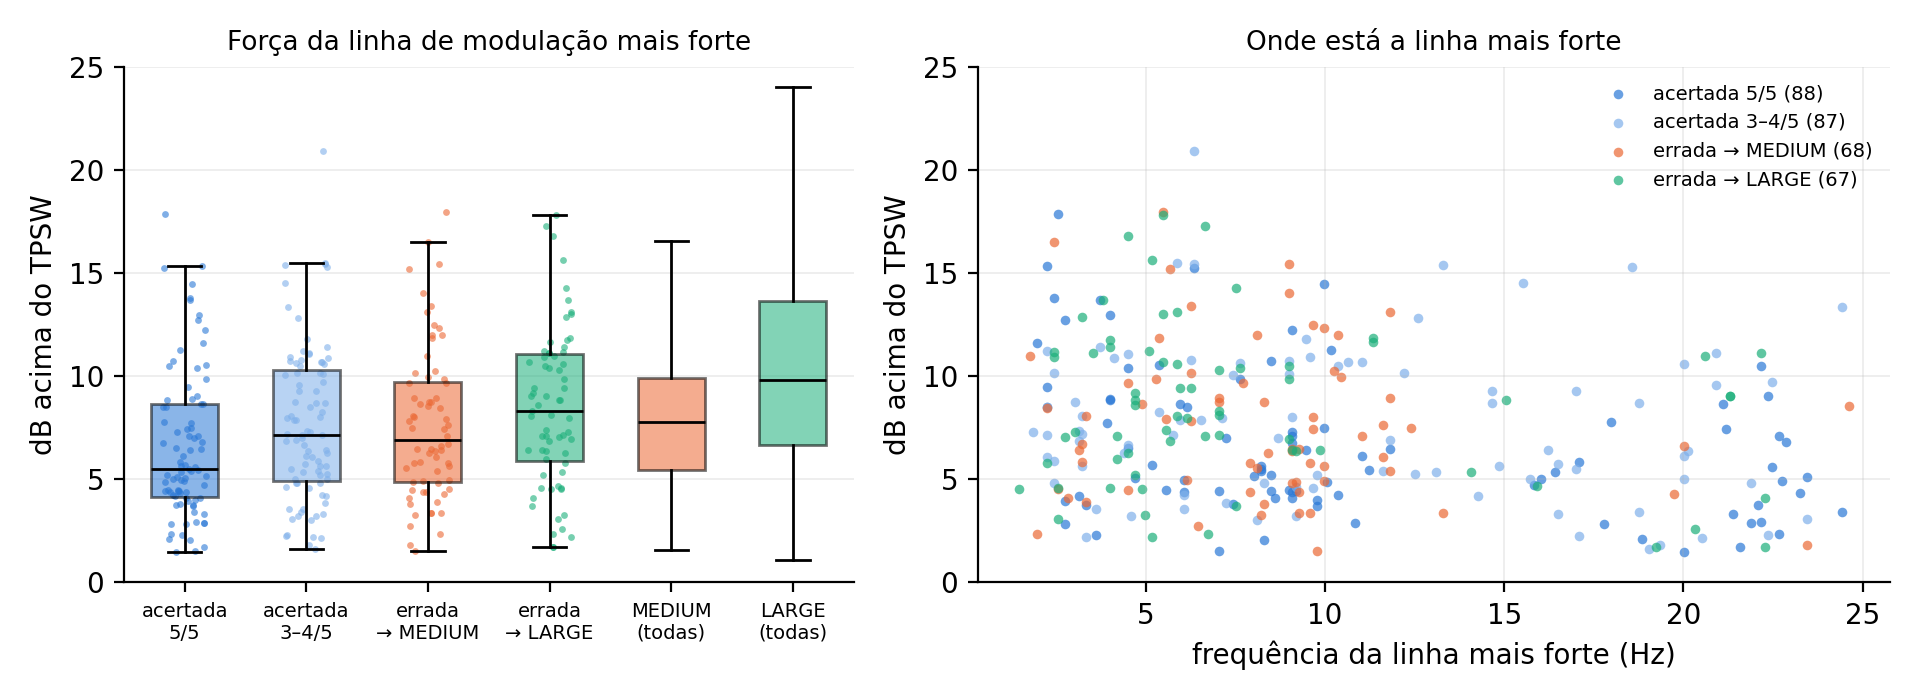
\includegraphics[width=0.86\textwidth]{demon_lanchas_pico.png}

    {\tiny Linha mais forte = máximo do DEMON acima do TPSW entre 1 e 25 Hz (abaixo de 1 Hz é resíduo da componente contínua).\par}
    \vspace{0.05cm}
    \begin{alertblock}{Leitura}
        \scriptsize
        \textbf{Erradas $\to$ LARGE têm linhas um pouco mais fortes} que as acertadas (mediana 8,3 $\times$ 5,5--7,1 dB; AUC 0,61, p = 0,008), na direção dos LARGE (9,8 dB). Erradas $\to$ MEDIUM não diferem (AUC 0,54). \textbf{Mas o efeito é fraco e não aparece dentro da mesma lancha} (AUC 0,54, p = 0,19), e a frequência da linha não separa os grupos. A linha forte do DEMON anda um pouco junto com o grave do LOFAR (Spearman 0,21): o DEMON parece não trazer uma pista nova sobre esses erros.
    \end{alertblock}
\end{frame}

\begin{frame}{As Mesmas Lanchas no MEL: Médias por Grupo}
    \begin{columns}[T]
        \begin{column}{0.50\textwidth}
            \centering
            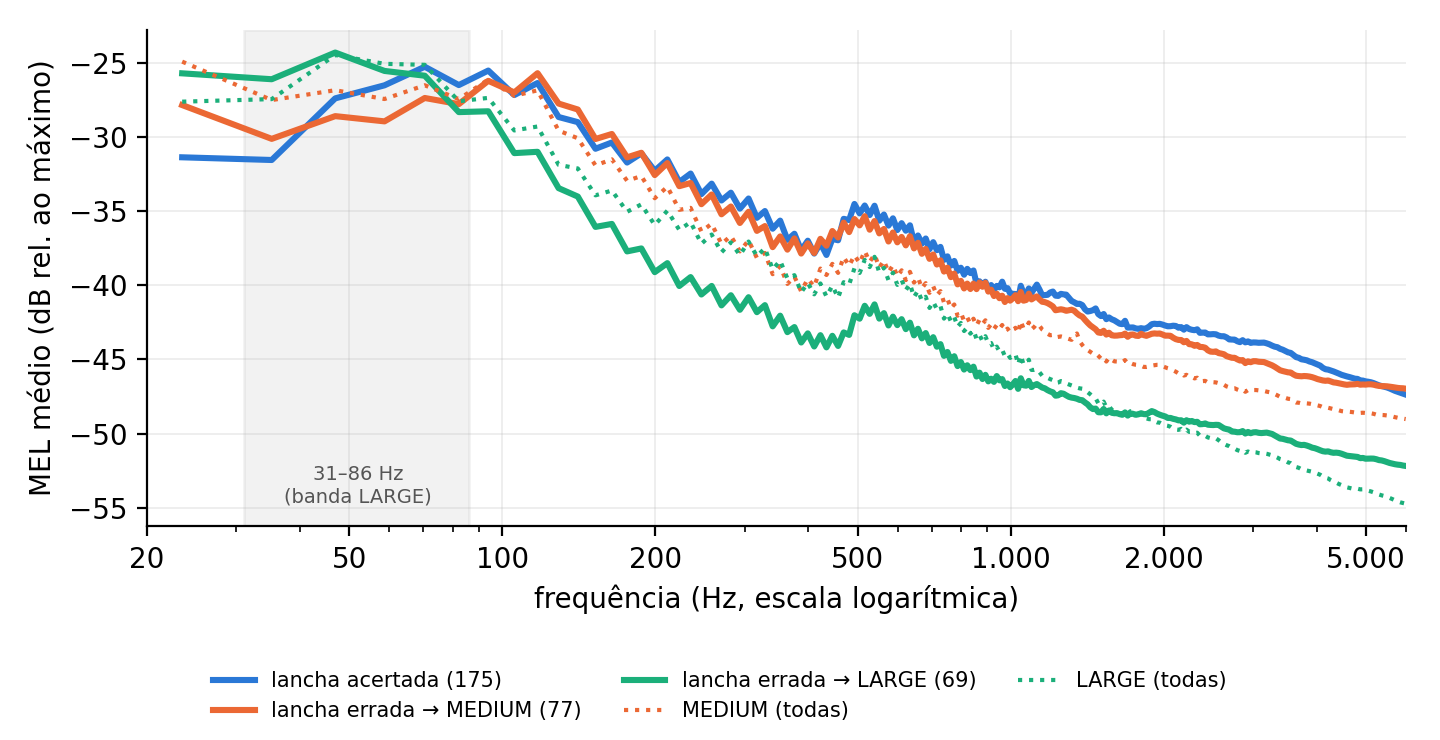
\includegraphics[width=\textwidth]{mel_lancha_espectro.png}\\[2pt]
            {\tiny Mesmos grupos (acertos/erros da MLP \textbf{LOFAR}). MEL do pipeline \textbf{sem normalização}: 256 bandas mel até 8 kHz, \textbf{sem TPSW}; eixo logarítmico, 20 Hz--6 kHz.\\
            \textbf{Eixo negativo:} dB relativo ao ponto mais forte da gravação (0 dB = máximo). \textbf{A queda com a frequência} é natural do ruído de navio; o MEL a mostra porque não usa TPSW.\par}
        \end{column}
        \begin{column}{0.48\textwidth}
            \begin{alertblock}{Leitura}
                \scriptsize
                \begin{itemize}
                    \setlength{\itemsep}{2pt}
                    \item \textbf{No grave (faixa cinza), as curvas quase se juntam:} as erradas $\to$ LARGE (verde) e as acertadas (azul) têm praticamente o mesmo nível.
                    \item \textbf{A diferença está do grave para cima:} a verde cai mais rápido a partir de 100 Hz. Em 1--6 kHz, fica $\sim$8 dB abaixo da azul, no nível da média LARGE (verde pontilhada). Em \textbf{72\% dos pares}, a errada tem menos agudo que a acertada.
                    \item \textbf{Erradas $\to$ MEDIUM (laranja)} ficam quase em cima das acertadas: o MEL não mostra por que elas erram.
                    \item O ``bico'' em $\sim$500 Hz aparece em todas as curvas, inclusive LARGE: não é próprio da lancha.
                \end{itemize}
            \end{alertblock}
        \end{column}
    \end{columns}
\end{frame}

\begin{frame}{Lanchas Erradas no MEL: Uma Linha por Gravação}
    \centering
    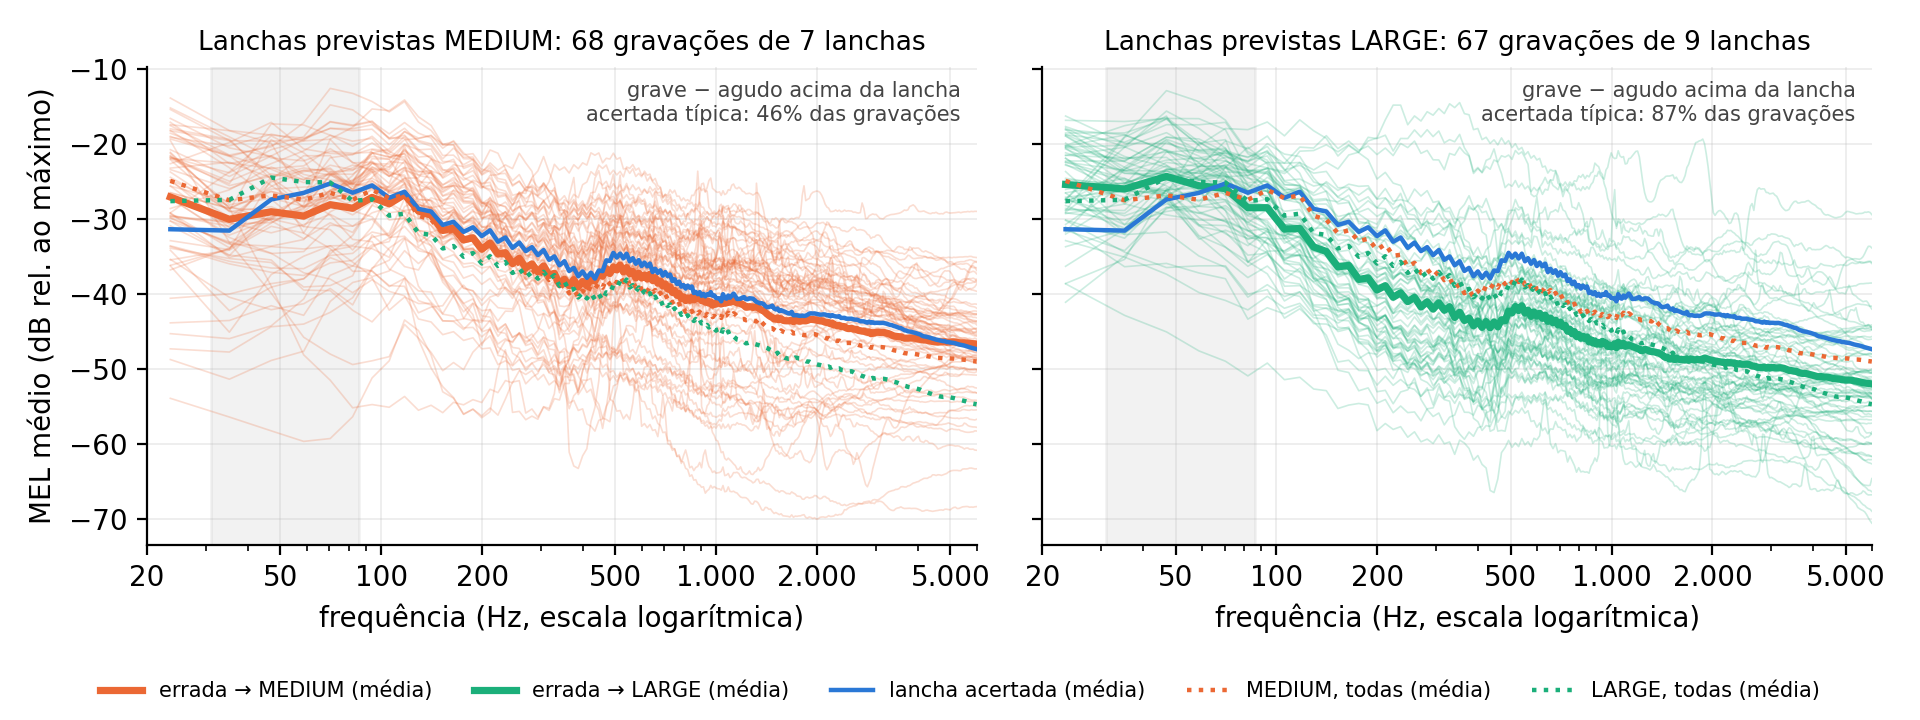
\includegraphics[width=0.86\textwidth]{mel_lanchas_erradas.png}

    {\tiny Grave $-$ agudo = média de 31--86 Hz menos média de 1--6 kHz (dB). Classe prevista como no slide das lanchas erradas no LOFAR.\par}
    \vspace{0.05cm}
    \begin{alertblock}{Leitura}
        \scriptsize
        \textbf{Erradas $\to$ LARGE:} 87\% têm o grave mais dominante sobre o agudo que a lancha acertada típica (23,6 $\times$ 17,4 dB; LARGE: 24,6). É a mesma pista do LOFAR vista de outro jeito: no LOFAR o grave se destaca do fundo; no MEL o agudo some. \textbf{Erradas $\to$ MEDIUM:} 46\%, como as acertadas; as curvas variam muito e não têm forma própria. Também no MEL não aparece uma corcova aguda de lancha.
    \end{alertblock}
\end{frame}

\begin{frame}{LOFAR $\times$ DEMON Dentro de Cada Lancha: Cada Gravação}
    \centering
    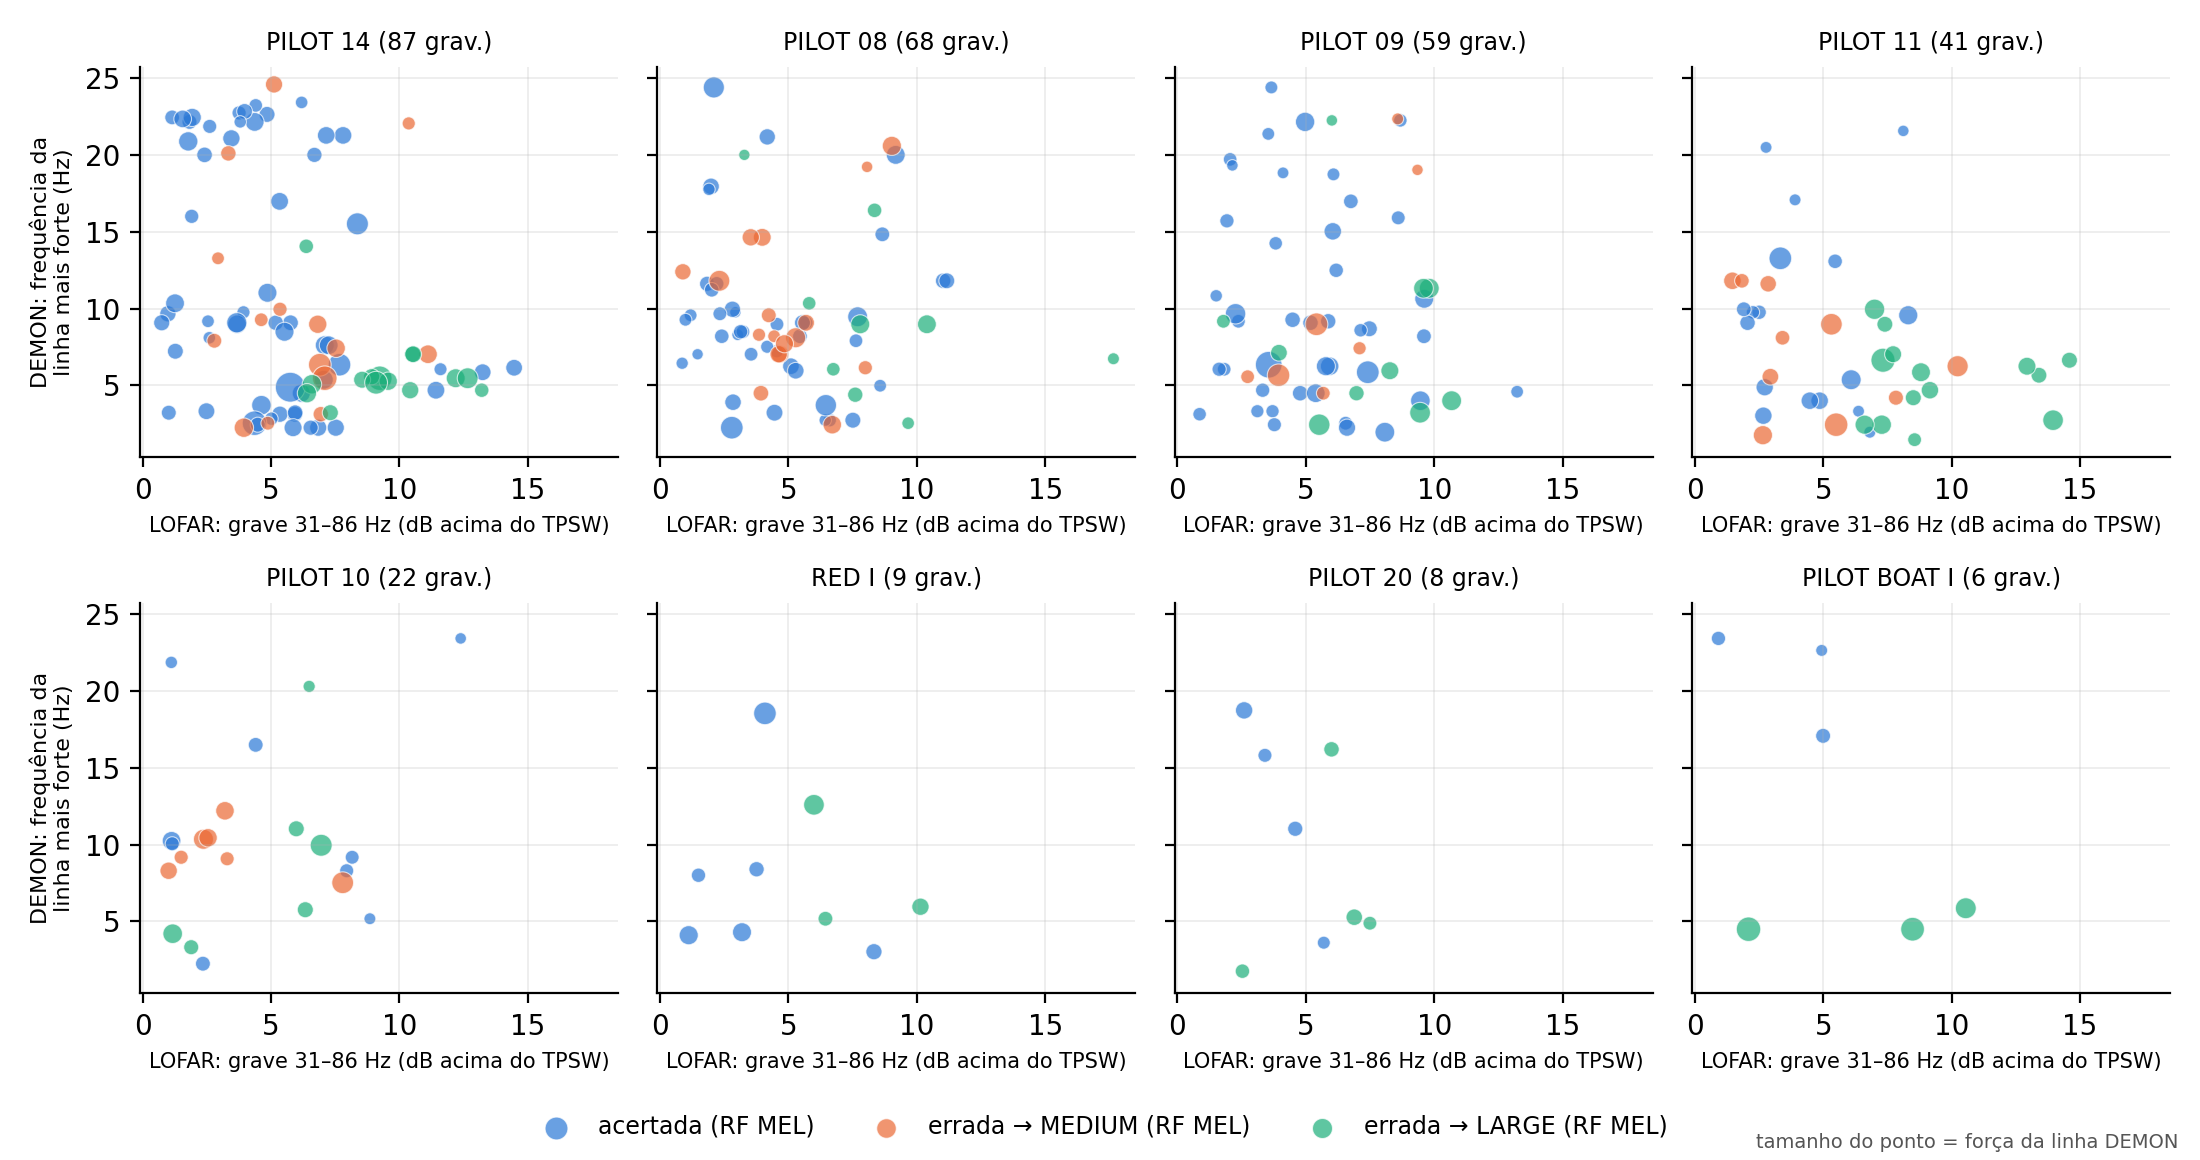
\includegraphics[width=0.62\textwidth]{lanchas_lofar_demon_rfmel.png}

    \vspace{-0.05cm}
    {\tiny \textbf{8 lanchas diferentes, um painel para cada}; cada ponto é \textbf{uma gravação daquela lancha}. Cor = o que a \textbf{RF MEL} fez com a gravação (o modelo com mais acerto de SMALL; \textbf{não usa o LOFAR}). \textbf{Eixo x:} LOFAR em 31--86 Hz, o ``grave'' típico dos LARGE. \textbf{Eixo y:} frequência da linha mais forte do DEMON (slide 41).\par}
    \begin{alertblock}{Leitura}
        \scriptsize
        Em quase todas as lanchas, os pontos verdes (tomadas por LARGE) ficam \textbf{à direita}: grave forte no LOFAR, que a RF MEL nunca viu. Na vertical (DEMON), as cores se misturam mais; os verdes só tendem a ficar um pouco mais embaixo ($\sim$5 Hz).
    \end{alertblock}
\end{frame}

\begin{frame}{Grupos de Outros Modelos: PILOT 14 em 6 Modelos}
    \centering
    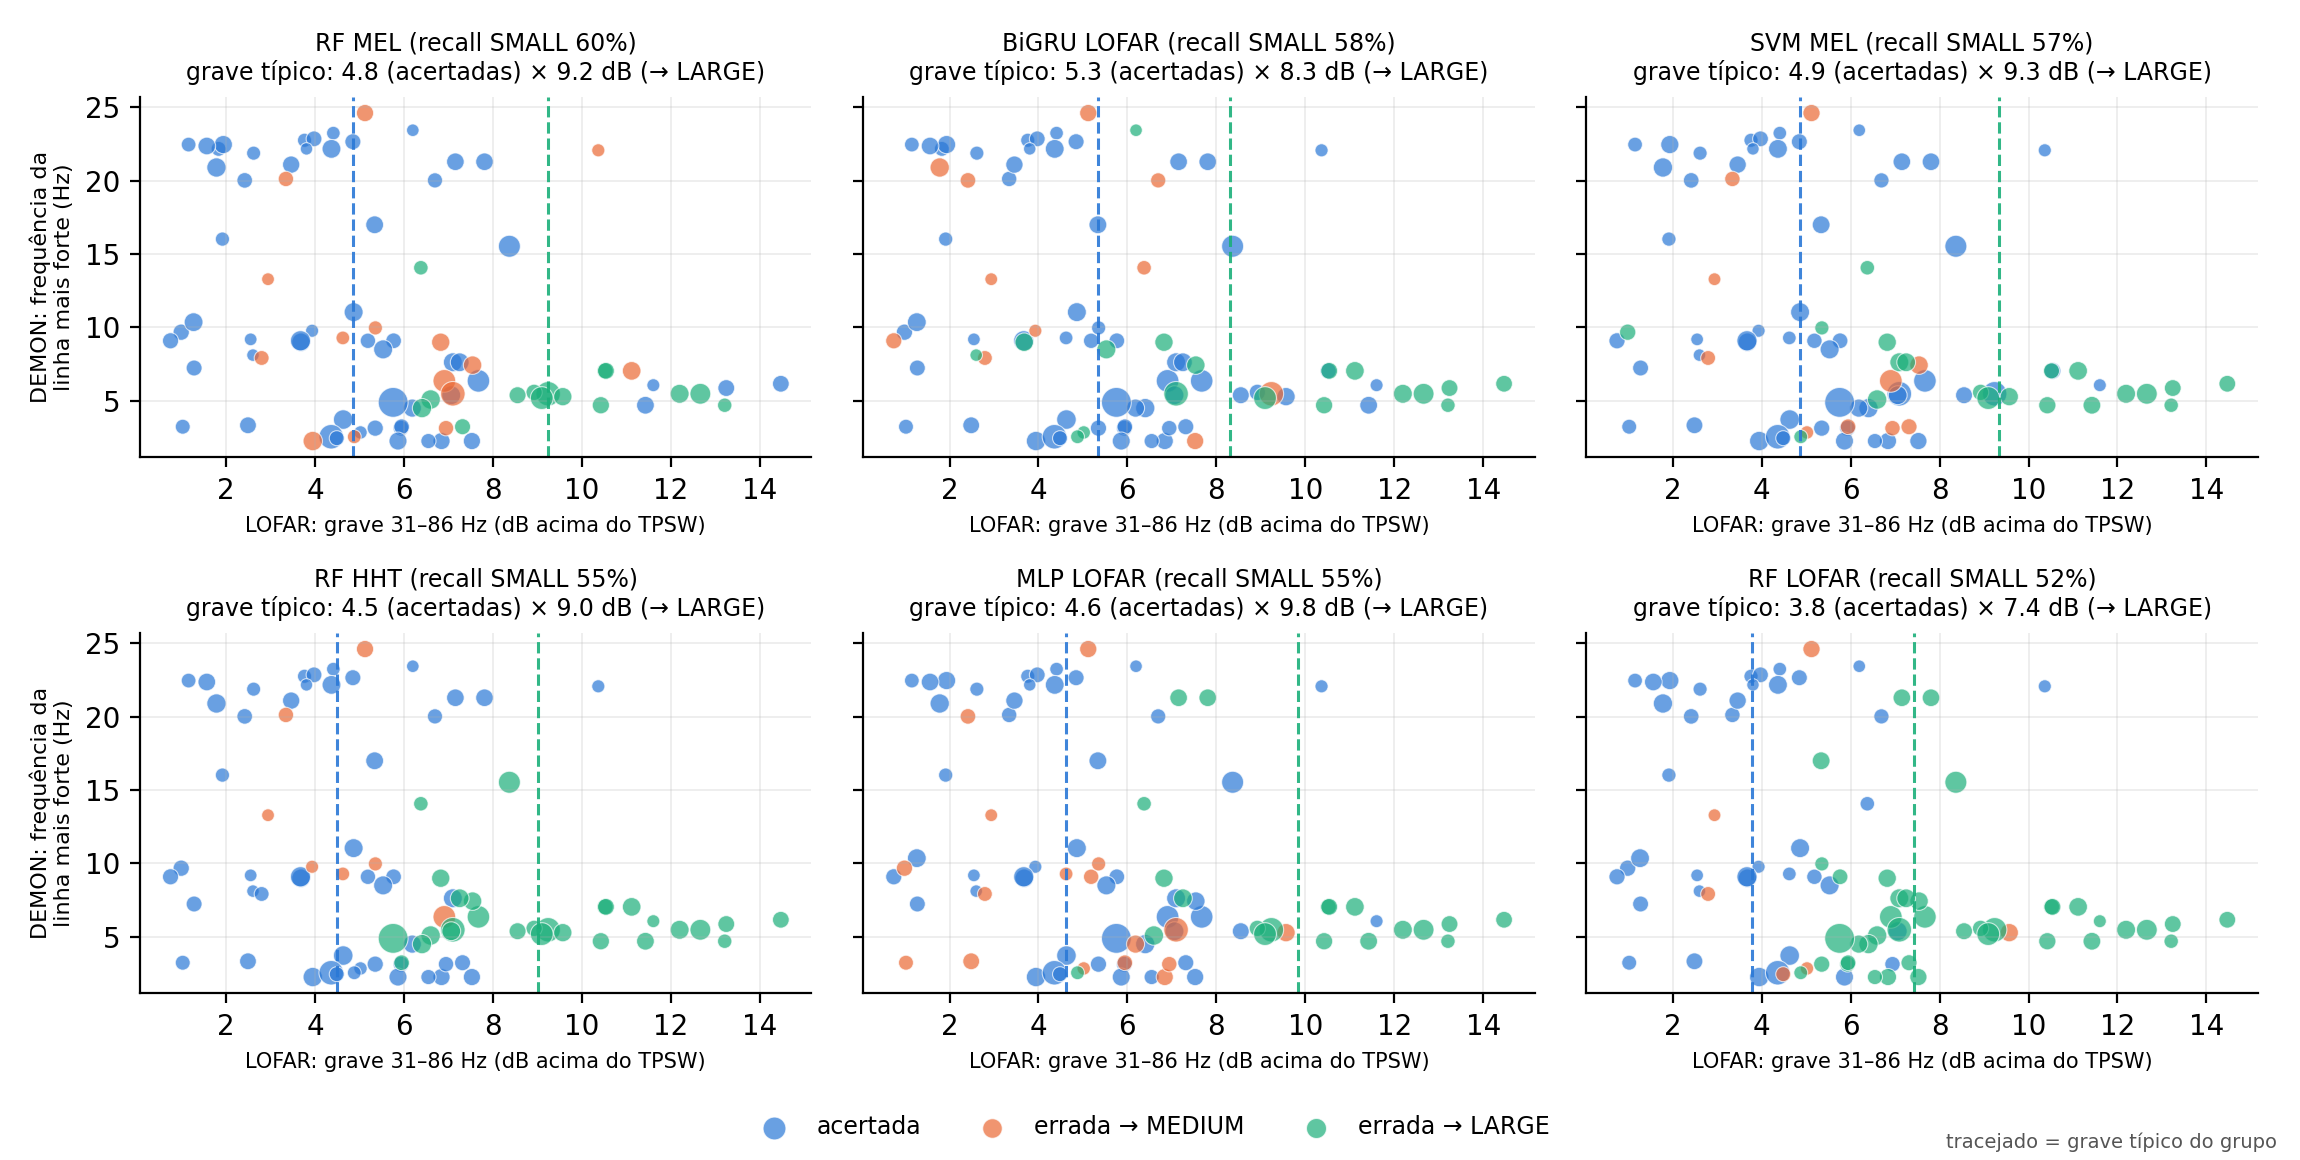
\includegraphics[width=0.64\textwidth]{lanchas_modelos_pilot14.png}

    \vspace{-0.05cm}
    {\tiny PILOT 14 (87 gravações), colorida por cada um dos \textbf{6 modelos com recall de SMALL acima de 50\%} (split por gravação). Entradas diferentes: MEL, LOFAR e HHT (este só vê 1--1.000 Hz, com outra matemática).\\
    \textbf{Grave} = energia média do LOFAR em 31--86 Hz de cada gravação (dB acima do fundo). \textbf{Grave típico} = mediana do grupo: metade das gravações tem grave abaixo, metade acima (linhas tracejadas).\par}
    \vspace{0.02cm}
    \begin{alertblock}{Leitura}
        \scriptsize
        Os modelos não erram exatamente as mesmas gravações, mas em todos o padrão se repete: as tomadas por LARGE têm grave típico de \textbf{7,4--9,8 dB}, contra \textbf{3,8--5,3 dB} das acertadas. Não é um efeito de um modelo só.
    \end{alertblock}
\end{frame}

\begin{frame}{Lanchas Tomadas por LARGE: O Que Podemos Concluir}
    \footnotesize
    \begin{columns}[T]
        \begin{column}{0.49\textwidth}
            \begin{block}{\small O que os dados indicam}
                \scriptsize
                \begin{enumerate}
                    \setlength{\itemsep}{2pt}
                    \item \textbf{O erro parece depender da gravação, não do modelo:} na mesma lancha, as gravações chamadas de LARGE são as de grave forte. Vale para 6 modelos e 3 entradas.
                    \item \textbf{Os modelos parecem associar ``grave forte'' a LARGE}, a assinatura dos LARGE (NB35), mas ela não é exclusiva: as lanchas erradas chegam a 7,4--9,8 dB, como um LARGE típico.
                    \item \textbf{Trocar de modelo ou de representação provavelmente não conserta}: todos erram de forma parecida. O augmentation também não ajudou.
                \end{enumerate}
            \end{block}
        \end{column}
        \begin{column}{0.49\textwidth}
            \begin{block}{\small O que não dá para concluir}
                \scriptsize
                \begin{enumerate}
                    \setlength{\itemsep}{2pt}
                    \item \textbf{Por que a lancha às vezes tem grave forte}: velocidade, manobra, distância? O IARA não registra.
                    \item \textbf{Que o grave é a única causa}: há sobreposição (AUC 0,75--0,90), e os erros para MEDIUM seguem sem explicação.
                    \item \textbf{Que a lancha está mais ``barulhenta''}: o LOFAR mede o grave contra o fundo vizinho, não o nível.
                    \item \textbf{Que o modelo decide por causa do grave}: é correlação.
                \end{enumerate}
            \end{block}
        \end{column}
    \end{columns}
    \vspace{0.05cm}
    \begin{alertblock}{\small Teste possível para provar a causa (sem treinar nada)}
        \scriptsize
        Nas lanchas tomadas por LARGE, \textbf{reduzir o grave de 31--86 Hz} ao nível das acertadas e passar de novo nos modelos treinados. Se virar SMALL, é o grave que puxa o erro.
    \end{alertblock}
\end{frame}

\begin{frame}{Lanchas: O Que Muda Dentro de Cada Lancha}
    \begin{columns}[c]
        \begin{column}{0.59\textwidth}
            \centering
            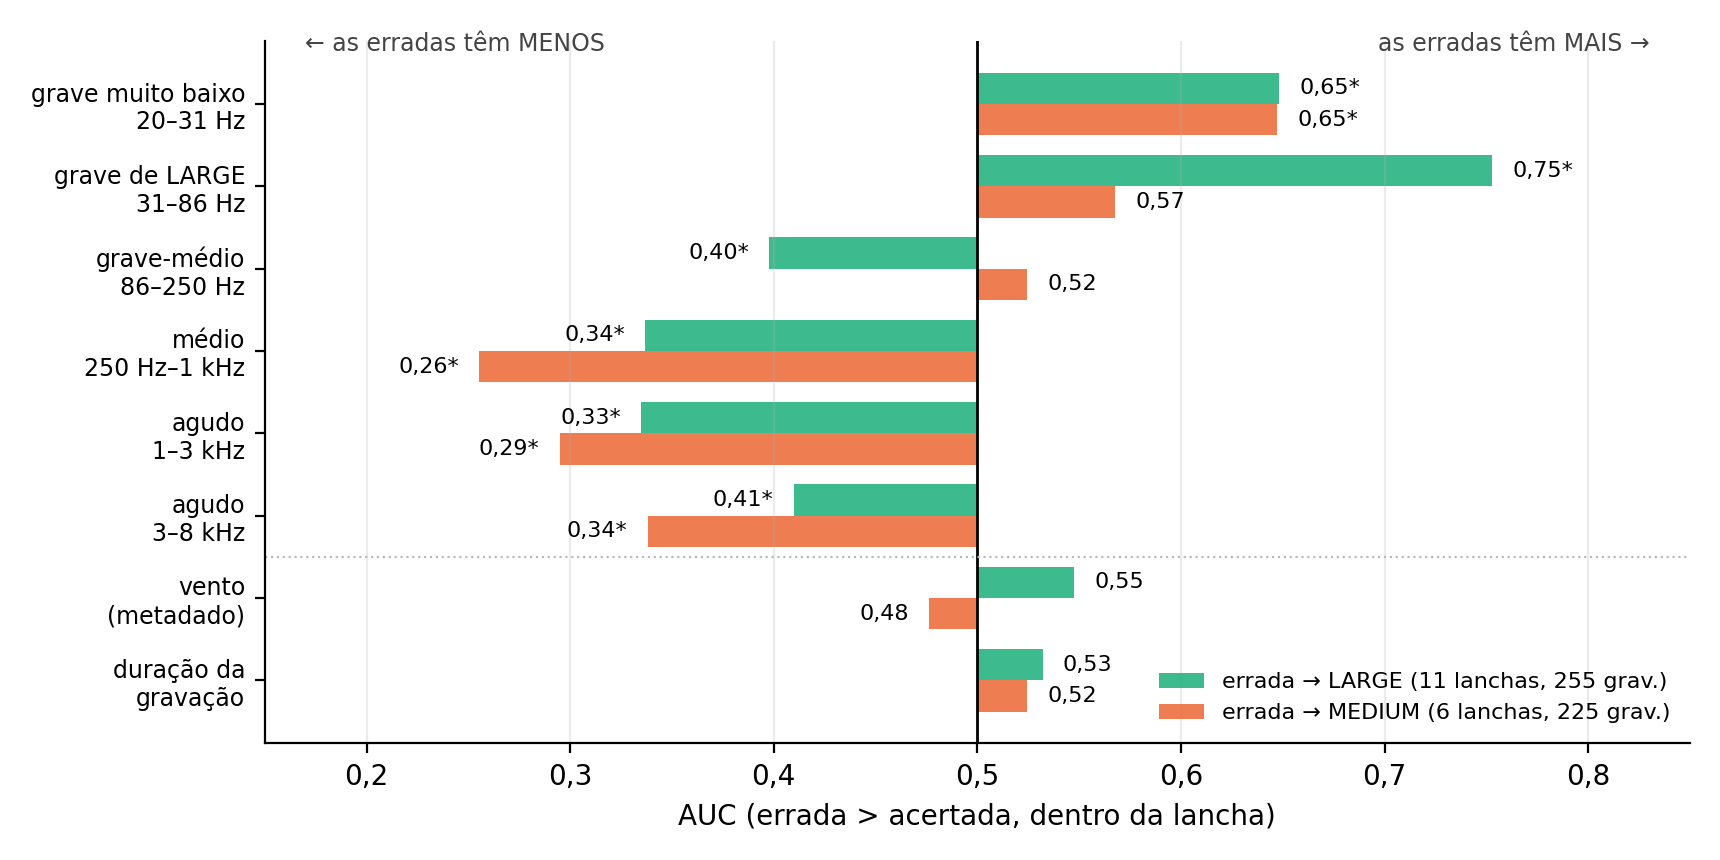
\includegraphics[width=\textwidth]{lanchas_o_que_muda.png}
        \end{column}
        \begin{column}{0.39\textwidth}
            \begin{block}{\small Como ler a AUC}
                \tiny
                \setlength{\tabcolsep}{2pt}
                \begin{tabular}{@{}lll@{}}
                \toprule
                Distância de 0,5 & Exemplos & Efeito \\
                \midrule
                até $\sim$0,05 & 0,45--0,55 & nenhum \\
                $\sim$0,05--0,15 & 0,35--0,45; 0,55--0,65 & fraco/moderado \\
                $\sim$0,15--0,25 & 0,25--0,35; 0,65--0,75 & moderado/forte \\
                $>$ $\sim$0,25 & $<$ 0,25; $>$ 0,75 & forte \\
                \bottomrule
                \end{tabular}\\[3pt]
                0,35 é tão forte quanto 0,65, só que no sentido contrário. * = p $<$ 0,05: não é acaso.
            \end{block}
        \end{column}
    \end{columns}

    {\tiny Grupos da RF MEL. Cada barra compara as gravações \textbf{erradas} com as \textbf{acertadas da mesma lancha}, numa faixa do LOFAR (dB acima do fundo). \textbf{Direita:} as erradas têm mais; \textbf{esquerda:} têm menos. Número = AUC (chance de uma errada ter valor maior).\par}
    \vspace{0.02cm}
    \begin{alertblock}{Leitura}
        \scriptsize
        \textbf{Nos dois tipos de erro}, menos linhas e bandas se destacam do fundo \textbf{acima de 250 Hz}, e 20--31 Hz se destaca mais (faixa que MEDIUM e LARGE têm mais que SMALL: pista de ``não-SMALL''). \textbf{O que diferencia os dois erros é o grave de 31--86 Hz}: \textbf{58\%} das tomadas por LARGE chegam ao grave de um LARGE típico (7,2 dB), contra \textbf{19\%} das acertadas. Vento e duração não mostraram relação.
    \end{alertblock}
\end{frame}

\begin{frame}{A Confusão Está Perto da Fronteira de 50 m?}
    \begin{columns}[c]
        \column{0.62\textwidth}
        \centering
        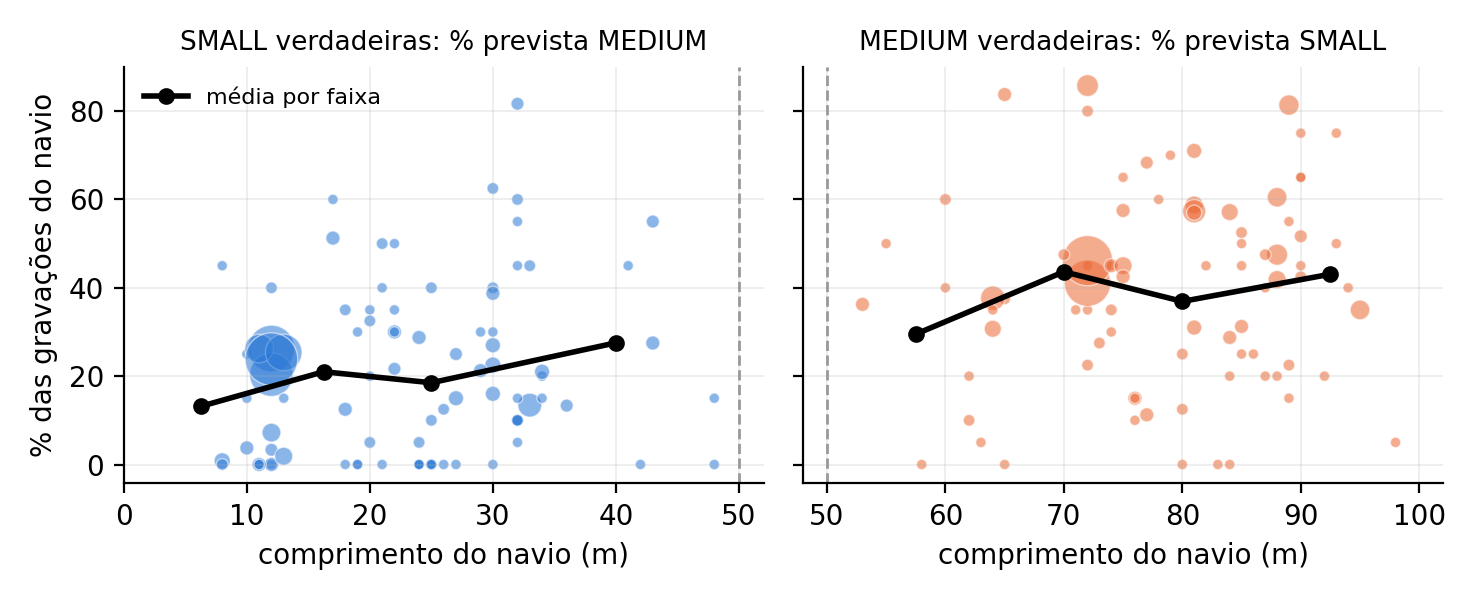
\includegraphics[width=\textwidth]{fronteira_comprimento.png}

        {\tiny Um ponto por navio (tamanho = nº de gravações); split por navio, média dos 4 modelos LOFAR.\par}
        \column{0.36\textwidth}
        \begin{block}{\small MEDIUM prevista SMALL}
            \scriptsize
            \centering
            \setlength{\tabcolsep}{3pt}
            \begin{tabular}{lc}
            \toprule
            Comprimento & \% \\
            \midrule
            50--65 m & 30 \\
            65--75 m & 44 \\
            75--85 m & 37 \\
            85--100 m & 43 \\
            \bottomrule
            \end{tabular}
        \end{block}
    \end{columns}
    \vspace{0.05cm}
    \begin{alertblock}{Leitura}
        \scriptsize
        \textbf{Em SMALL}, os barcos maiores vão um pouco mais para MEDIUM (13\% até 15 m; 21--26\% de 15 a 50 m), mas a subida não é significativa (p = 0,11), não se concentra perto de 50 m e pode ser efeito do \textbf{tipo}: as menores são lanchas, que quase nunca vão para MEDIUM. \textbf{Em MEDIUM, não há sinal de fronteira}: os mais curtos (50--65 m) são os que \textbf{menos} viram SMALL. O acerto de MEDIUM também não muda com o comprimento (25--32\% em todas as faixas).
    \end{alertblock}
\end{frame}

%===========================================
% SEÇÃO 8
%===========================================
\section{Data Augmentation}

\begin{frame}
    \centering
    \huge Data Augmentation
\end{frame}

\begin{frame}{Sete Variantes Testadas no LOFAR}
    \footnotesize
    \begin{table}
    \centering
    \scriptsize
    \setlength{\tabcolsep}{4pt}
    \begin{tabular}{lll}
    \toprule
    Variante & O que faz & O que simula \\
    \midrule
    navio & peso igual por navio (reponderação) & tirar o domínio das lanchas e das HANG BO \\
    stretch & estica o eixo de frequência (0,92--1,08) & outra rotação/velocidade \\
    mask & apaga 2 faixas de até $\sim$375 Hz & não depender de uma raia \\
    mixnavio & mistura 2 navios da mesma classe & ``navios virtuais'' \\
    ruido & ruído gaussiano no LOFAR padronizado & outra condição (simplificado) \\
    \textbf{bg} & \textbf{soma gravação real de BACKGROUND ao áudio} & \textbf{o mesmo navio em outro mar} \\
    & \textbf{e recalcula o LOFAR} & \\
    \bottomrule
    \end{tabular}
    \end{table}
    \vspace{0.05cm}
    \begin{block}{\small Como foi testado}
        \scriptsize
        Split por navio, mesmos folds, sementes e modelo da base; o teste é sempre o LOFAR original. \textbf{Na bg}: 4 cópias por gravação, fundo 0--20 dB abaixo da gravação, e só valem fundos do treino do fold (2 cópias válidas, em média). O LOFAR usado pelos modelos não foi alterado (pasta própria \texttt{lofar\_mixbg}).
    \end{block}
    \begin{alertblock}{Critério de ganho real (definido antes dos resultados)}
        \scriptsize
        $\Delta$ ACC $\geq$ +1,5 ponto, p $<$ 0,05 (teste F 5x2cv, o mesmo do artigo) e melhora em $\geq$ 8 de 10 folds, sem SMALL e MEDIUM se moverem em sentidos opostos.
    \end{alertblock}
\end{frame}

\begin{frame}{MLP LOFAR: Nenhuma Variante Melhora}
    \footnotesize
    \begin{table}
    \centering
    \scriptsize
    \setlength{\tabcolsep}{4pt}
    \begin{tabular}{lcccccccc}
    \toprule
    Variante & ACC & SMALL & MEDIUM & LARGE & BG & $\Delta$ ACC & p (F 5x2cv) & folds melhores \\
    \midrule
    base & 58,7 & 49,4 & 36,0 & 68,7 & 80,8 & -- & -- & -- \\
    navio & 57,4 & \calo{32,3} & 39,2 & 75,9 & 82,0 & $-$1,35 & 0,16 & 4 \\
    stretch & 58,2 & 42,1 & 41,7 & 62,6 & 86,5 & $-$0,52 & 0,60 & 3 \\
    mask & 57,8 & 32,4 & 45,6 & 71,5 & 81,7 & $-$0,94 & 0,23 & 3 \\
    mixnavio & 59,0 & 45,7 & 38,8 & 66,2 & 85,2 & +0,26 & 0,60 & 8 \\
    ruido & 57,8 & 44,3 & 40,1 & 66,3 & 80,4 & $-$0,94 & 0,47 & 3 \\
    navio+stretch+mask & 56,0 & \calo{13,8} & \camd{61,5} & 65,3 & 83,3 & \calo{$-$2,74} & \calo{0,03} & 2 \\
    bg & 58,2 & 50,0 & 34,9 & 66,8 & 81,3 & $-$0,48 & 0,59 & 2 \\
    \bottomrule
    \end{tabular}
    \end{table}
    {\tiny ACC = acurácia balanceada (média dos 4 recalls), métrica principal no split por navio porque o SP pode zerar num fold.\par}
    \vspace{0.1cm}
    \begin{alertblock}{Leitura}
        \scriptsize
        A melhor (mixnavio, +0,26) está dentro da variação entre treinos. A única significativa é uma \textbf{piora}: navio+stretch+mask leva MEDIUM a 62\% e derruba SMALL a 14\%; o modelo parece ter passado a responder ``MEDIUM'' na dúvida. \textbf{Peso por navio derruba SMALL}: o padrão das lanchas de prático parece sustentar o recall SMALL.
    \end{alertblock}
\end{frame}

\begin{frame}{E em Outros Modelos? RF, SVM e BiGRU}
    \begin{columns}[c]
        \column{0.62\textwidth}
        \centering
        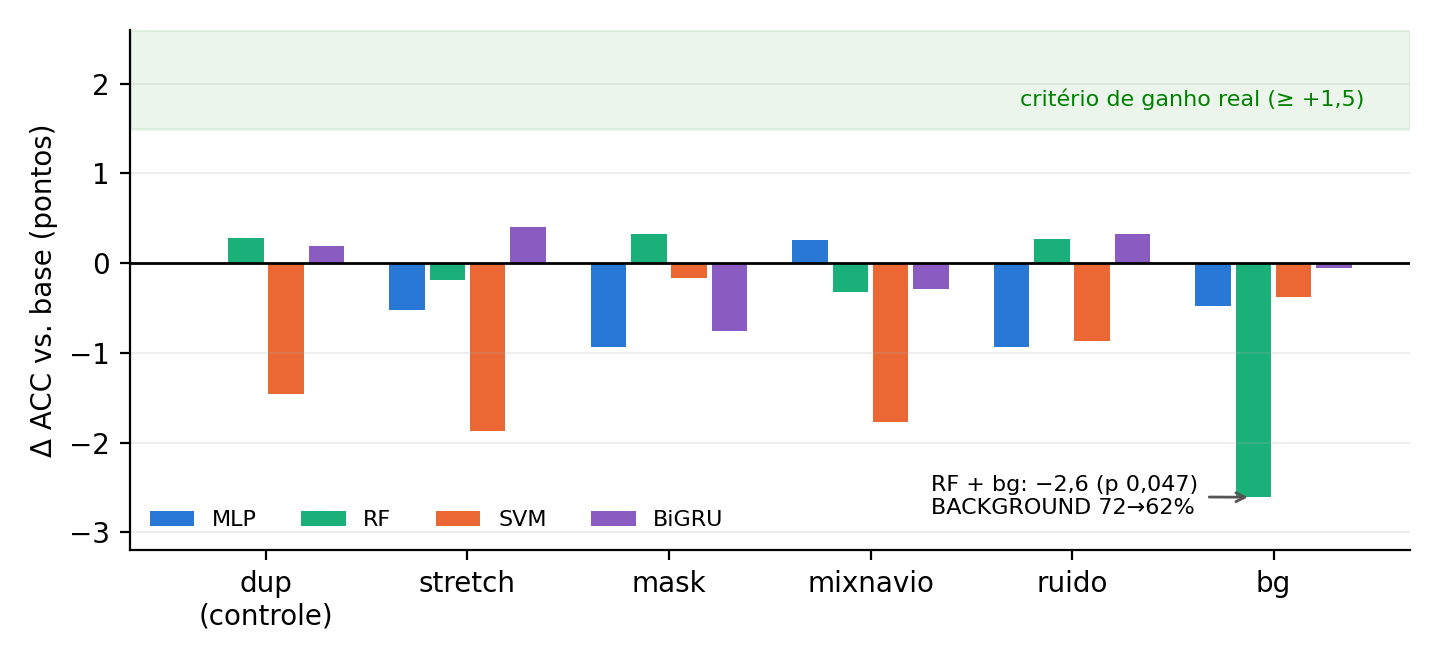
\includegraphics[width=\textwidth]{aug_modelos.png}
        \column{0.36\textwidth}
        \begin{block}{\small Como foi feito}
            \tiny
            Mesmos modelos, hiperparâmetros e folds do NB29. Cada gravação de treino ganha 1 versão modificada. \textbf{dup} = cópia idêntica: mostra o efeito de só dobrar o treino.
        \end{block}
        \begin{block}{\small ACC da base}
            \tiny
            MLP 58,7 \quad RF 52,7 \quad SVM 56,2 \quad BiGRU 53,8
        \end{block}
    \end{columns}
    \vspace{0.05cm}
    \begin{alertblock}{Leitura}
        \scriptsize
        \textbf{Nenhum modelo melhora.} O maior ganho é +0,4 (BiGRU + stretch), do tamanho do controle dup. No SVM, as variantes só trocam SMALL por MEDIUM. A única diferença significativa é a piora do RF com bg: com mar real nas gravações de navio, ele provavelmente passa a confundir mar sem navio com navio. \textbf{CNN do artigo não foi rodada} ($\sim$60 h por variante).
    \end{alertblock}
\end{frame}

\begin{frame}{O Modelo Usa o ``Ambiente'' da Gravação?}
    \footnotesize
    \begin{block}{\small Assinatura de ambiente}
        \scriptsize
        O IARA não registra data, sessão nem hidrofone. Usei o espectro do \textbf{bloco de 10 s mais silencioso} de cada gravação, em \textbf{8--23 kHz} (fora da faixa do LOFAR).
    \end{block}
    \begin{columns}[t]
        \column{0.46\textwidth}
        \begin{block}{\small T1: o ambiente indica a classe?}
            \scriptsize
            SMALL $\times$ MEDIUM só pelo ambiente, em navios novos: \textbf{AUC 0,51--0,58} (acaso 0,50). Quase não indica.
        \end{block}
        \column{0.52\textwidth}
        \begin{block}{\small T2: a previsão segue o ambiente?}
            \scriptsize
            \centering
            \setlength{\tabcolsep}{3pt}
            \begin{tabular}{lcc}
            \toprule
            Ambiente parecido com o da outra classe & base & bg \\
            \midrule
            SMALL: queda no acerto (pontos) & 19 & 21 \\
            MEDIUM: queda no acerto (pontos) & 13 & 15 \\
            \bottomrule
            \end{tabular}

            {\tiny SMALL com ambiente de MEDIUM no treino: 38\% de acerto, contra 58\%.\par}
        \end{block}
    \end{columns}
    \vspace{0.1cm}
    \begin{alertblock}{Leitura}
        \scriptsize
        O ambiente da gravação \textbf{mexe na decisão} do modelo, mas misturar mar real (bg) \textbf{não reduz o efeito}. Então provavelmente não é ruído de fundo somado: pode ser algo da própria gravação (distância, velocidade, cadeia de gravação), que o IARA não registra.
    \end{alertblock}
\end{frame}

%===========================================
% SEÇÃO 9
%===========================================
\section{Conclusões e Próximos Passos}

\begin{frame}
    \centering
    \huge Conclusões e Próximos Passos
\end{frame}

\begin{frame}{Conclusões}
    \footnotesize
    \begin{block}{\small O que os experimentos mostram}
        \scriptsize
        \begin{enumerate}
            \setlength{\itemsep}{2pt}
            \item \textbf{Há uma tendência de o gargalo ser o número de navios distintos}: $\sim$12 navios efetivos por classe, curva subindo sem estabilizar.
            \item \textbf{O SP do artigo provavelmente superestima MEDIUM}: boa parte dos 66\% parece vir de navios repetidos (HANG BO); em navios novos, 28--35\%.
            \item \textbf{LARGE e BACKGROUND generalizam}: o LARGE quase não perde em navios novos, e o BACKGROUND acerta 70--81\% de gravações nunca vistas. O acerto do LARGE acompanha o grave em $\sim$50 Hz, que não é exclusivo dele.
            \item \textbf{SMALL tem um problema a mais}: as lanchas tomadas por LARGE têm grave de LARGE, em 6 modelos; o erro parece vir da gravação.
            \item \textbf{SMALL $\times$ MEDIUM não parece ser física de fronteira}: a confusão não se concentra perto de 50 m e pode acompanhar o \textbf{tipo} de navio, não o tamanho.
            \item \textbf{Augmentation não compensou a falta de navios} (7 variantes, 4 modelos).
        \end{enumerate}
    \end{block}
    \begin{alertblock}{\small Ressalvas}
        \scriptsize
        Os LARGE foram gravados com o mar mais calmo (viés da base). A origem dos graves nas lanchas exige metadados que o IARA não publica (velocidade, distância, hidrofone).
    \end{alertblock}
\end{frame}

\begin{frame}{Próximos Passos}
    \footnotesize
    \begin{columns}[T]
        \begin{column}{0.49\textwidth}
            \begin{block}{\small Fora do IARA: tamanho dentro do mesmo tipo}
                \scriptsize
                \textbf{UniqueShip} (Ocean Networks Canada, 2026): 4.218 navios, $\sim$3.500 h, comprimento pelo AIS em cada trecho, folds por navio.
                \begin{itemize}
                    \setlength{\itemsep}{1pt}
                    \item 1.280 navios $<$ 50 m, só 69 entre 50 e 100 m, 2.859 $\geq$ 100 m: \textbf{não serve para SMALL $\times$ MEDIUM}.
                    \item Mas tem \textbf{286 rebocadores de 10 a 50 m}, 227 pesqueiros e 393 barcos de recreio.
                    \item Pergunta: \textbf{dentro dos rebocadores, o LOFAR prevê o comprimento?} Se sim, há pista acústica de tamanho; se não, o que se aprende é o tipo.
                    \item Também serve para repetir fora do IARA a busca por uma pista de barco pequeno.
                \end{itemize}
            \end{block}
        \end{column}
        \begin{column}{0.49\textwidth}
            \begin{block}{\small No IARA}
                \scriptsize
                \begin{itemize}
                    \setlength{\itemsep}{1pt}
                    \item \textbf{Analisar melhor o HHT}: olhar gravação a gravação, por tipo e dentro de cada navio, como fizemos com LOFAR, MEL e DEMON.
                    \item Solicitar ao PMPAS-BS \textbf{gravações mais recentes}: ver se hoje há mais diversidade de navios, sobretudo SMALL e MEDIUM de outros tipos (rebocadores e pesqueiros maiores, barcos de apoio menores), o que permitiria separar tipo de tamanho.
                    \item Solicitar também distância, observatório e calibração: permitiriam usar o nível de fonte, a medida física mais direta de porte.
                \end{itemize}
            \end{block}
        \end{column}
    \end{columns}
\end{frame}

\end{document}
